\documentclass[12pt,c, german, aspectratio=169]{beamer} % t: top alignment % handout option
\newcommand{\englishSlides}{}
%\newcommand\noSolutions{}
%% modularization
\newcommand{\topicbasepath}{}
\newcommand{\topicpath}{}
\newcommand{\settopicbasepath}[1]{\renewcommand{\topicbasepath}{#1}}
\newcommand{\settopicpath}[1]{\renewcommand{\topicpath}{#1}}
\newcommand{\importfrompath}[1]{\import{\topicbasepath\topicpath}{#1}}

\newcommand{\CodeInput}[1]{\VerbatimInput[frame=lines, fontfamily=courier,fontseries=b,fontsize=\footnotesize]{\topicbasepath\topicpath progs/#1}}
\newcommand{\textattachcode}[2]{\textattachfile[color=1 0 0]{\topicbasepath\topicpath progs/#1}{#2}}
\newcommand{\CodeInputFormatted}[1]{\lstinputlisting[style=normal,basicstyle={\srcfont\footnotesize}]{\topicbasepath\topicpath progs/#1}}
\graphicspath{{img/}{..}{}{}}{}



% Python-specific
\newcommand{\pythonerror}[2]{{\darkred\lstinline"#1:"} {\black\lstinline"#2"}}


\newcommand{\python}[1]{\lstinline"#1"}
\newcommand{\pythonkey}[1]{{\fcb\lstinline"#1"}}

\newcommand{\beginlst}{\begin{lstlisting}[language=Python,style=normal,escapechar=?,morekeywords={True, False}, mathescape]}


%% Reduce the amount of output LaTeX generates.
%% This makes it slightly easier to find errors, if any occur.
\makeatletter
\renewcommand{\PackageInfo}[2]{} %% Remove package information
\renewcommand{\@font@info}[1]{}  %% Remove font information
\renewcommand{\@latex@info}[1]{} %% Remove LaTeX information
\makeatother

% This is the theme we are using for the slides
% the theme file contains any information relevant for the design and look of the slides
\usetheme{Lecture}

\usepackage[english]{babel}
\usepackage[utf8]{inputenc}
\usepackage[T1]{fontenc}

\usepackage{graphicx}
\usepackage{transparent} %% Provides \transparent

\usepackage{hyperref}
\usepackage[export]{adjustbox}
\usepackage{varwidth}
\usepackage{fancyvrb}
\usepackage[normalem]{ulem}

\usepackage{bbm}

% -------------- tikz ----------------------
\usepackage{tikz}
\usetikzlibrary{calc,shapes,shadows,patterns,decorations.pathreplacing,matrix,fit,shapes.geometric,shapes.multipart,fit,chains,scopes,overlay-beamer-styles,mindmap}
% TIKZ 
\usetikzlibrary{arrows,arrows.meta,positioning}
\usetikzlibrary{shapes.symbols}
\usetikzlibrary{fit,backgrounds}
\usetikzlibrary{shadows}
\usetikzlibrary{trees}
\usetikzlibrary{automata}
% For instance smilies: \Smiley and some nice symbols (WinDings)
\usepackage{tikzsymbols}
\usepackage{pifont}


\usepackage{comment} % for being able to uncomment sections of the slides for different lectures

\usepackage{etoolbox}
\usepackage[vlined]{algorithm2e}

\usepackage{xifthen}
\usepackage{xstring}
\usepackage{xpatch}
\usepackage{xsavebox}

\usepackage{booktabs}
\usepackage{colortbl}
\usepackage{pbox}

% tables and arrays 
\usepackage{array}
\newcolumntype{M}[1]{>{\centering\arraybackslash}m{#1}}
\newcolumntype{P}[1]{>{\centering\arraybackslash}p{#1}}

\usepackage{attachfile}
\setcounter{atfi@tmp}{0} % in order to avoid a running counter during latexmk


% ----- additional vertical spaces in itemize -----
\setbeamertemplate{itemize/enumerate subbody begin}{\vspace{1ex}}
\setbeamertemplate{itemize/enumerate subbody end}{\vspace{1ex}}

% itemize with left aligned itemize items
\newenvironment{bullets}{%
\settowidth{\leftmargini}{\usebeamertemplate{itemize item}}
\addtolength{\leftmargini}{\labelsep}
\addtolength{\itemsep}{0.5ex}
\itemize[]}
{\enditemize}


\newcommand{\srcfont}{\usefont{T1}{lmtt}{b}{n}}
% narrow font for code
\newcommand{\srcfontn}{\usefont{T1}{lmvtt}{b}{n}}
% font for verbatim environment. Note: must be fixed width!
\fvset{fontfamily=lmtt, fontseries=b%,formatcom=\color{fcb}
}

% ----------------- SPACING -----------------------

\newcommand*{\addVerticalSpace}[1]{%
  \ifvmode%
    %% We are already in vertical mode
  \else%
    \par% %% Switch to vertical mode
    \vspace{-\baselineskip}% %% Undo most vertical space due to preceding \par ...
    \vspace{\lineskip}% %% ... but not all
  \fi%
  \ifdim#1>0pt%
    \addvspace{#1}% %% Positive vertical space with \addvspace
  \else%
    \vspace{#1}% %% \addvspace doesn't support negative vertical space
  \fi%
}

\newcommand*{\tinysep}{\addVerticalSpace{0.5em}}
\newcommand*{\smallsep}{\addVerticalSpace{0.75em}}
\newcommand*{\medsep}{\addVerticalSpace{1.0em}}
\newcommand*{\bigsep}{\addVerticalSpace{1.5em}}
\newcommand*{\largesep}{\addVerticalSpace{2em}}

\newcommand*{\negtinysep}{\addVerticalSpace{-0.5em}}
\newcommand*{\negsmallsep}{\addVerticalSpace{-0.75em}}
\newcommand*{\negmedsep}{\addVerticalSpace{-1.0em}}
\newcommand*{\negbigsep}{\addVerticalSpace{-1.5em}}
\newcommand*{\neglargesep}{\addVerticalSpace{-2.0em}}

% ----------------- COLORS -----------------------

%%% Some colors from https://jfly.uni-koeln.de/color/ (colorblind barrier-free color pallet)
\definecolor{black}{RGB}{0,0,0}
\definecolor{orangeCUD}{RGB}{230,159,0}
\definecolor{skyblueCUD}{RGB}{86,180,233}
\definecolor{blueCUD}{RGB}{0,114,178}
%\definecolor{blueCUD}{RGB}{255,0,0}
\definecolor{greenCUD}{RGB}{0,158,115}
\definecolor{yellowCUD}{RGB}{240,228,66}
\definecolor{redCUD}{RGB}{213,94,0}
\definecolor{purpleCUD}{RGB}{204,121,167}


%%% Some colours, from https://en.wikibooks.org/wiki/LaTeX/Colors
\definecolor{plum}{HTML}{92268F}
\definecolor{royalpurple}{HTML}{613F99}
\definecolor{redorange}{HTML}{F26035}
\definecolor{forestgreen}{HTML}{009B55}
\definecolor{olivegreen}{HTML}{3C8031}

\definecolor{lightred}{rgb}{1,0.5,0.5}
\colorlet{slidebg}{white!95!black}

\definecolor{lightblue}{RGB}{200,200,250}

\definecolor{lightgreen}{RGB}{173,255,47}
\definecolor{lightorange}{RGB}{255,165,0}
\definecolor{boxcolor}{RGB}{200,200,200}
\definecolor{darkgreen}{named}{olivegreen}

\definecolor{fig}{named}{blue}


%% orange
\definecolor{bca}{RGB}{230,159,0}
\newcommand{\bca}{\color{orangeCUD}}
\definecolor{fca}{RGB}{230,159,0}
\newcommand{\fca}{\color{orangeCUD}}


%% blue
\definecolor{bcb}{RGB}{86,180,233} %86,180,233
\newcommand{\bcb}{\color{skyblueCUD}}
%\newcommand{\bcb}{\color{bcb}}
\definecolor{fcb}{RGB}{0,114,178}
\newcommand{\fcb}{\color{blueCUD}}
%\newcommand{\fcb}{\color{fcb}}
%% green
\definecolor{bcc}{RGB}{0,158,115}
\newcommand{\bcc}{\color{greenCUD}}
\definecolor{fcc}{RGB}{0,158,115}
\newcommand{\fcc}{\color{greenCUD}}

%% red
\definecolor{bcd}{RGB}{213,94,0}
\newcommand{\bcd}{\color{redCUD}}
\definecolor{fcd}{RGB}{213,94,0}
\newcommand{\fcd}{\color{redCUD}}

%% purple
\definecolor{bce}{RGB}{204,121,167}
\newcommand{\bce}{\color{purpleCUD}}
\definecolor{fce}{RGB}{204,121,167}
\newcommand{\fce}{\color{purpleCUD}}

%% yellow
\definecolor{bcf}{RGB}{240,228,66}
\newcommand{\bcf}{\color{yellowCUD}}
\definecolor{fcf}{RGB}{240,228,66}
\newcommand{\fcf}{\color{yellowCUD}}


%% grey
\definecolor{bcg}{RGB}{230,230,230}
\newcommand{\bcg}{\color{black!30}}
\definecolor{fcg}{RGB}{230,230,230}
\newcommand{\fcg}{\color{black!30}}
\newcommand{\bc}{\color{black!30}}
\definecolor{bc}{RGB}{230,230,230}
\newcommand{\grey}{\color{black!30}}
\definecolor{grey}{RGB}{230,230,230}
\newcommand{\black}{\color{black}}

% dark red
\definecolor{darkred}{RGB}{139,0,0}
\newcommand{\darkred}{\color{darkred}}

% dark blue
\definecolor{darkblue}{RGB}{0,0,139}
\newcommand{\darkblue}{\color{darkblue}}


\definecolor{textbg}{named}{white}
\definecolor{textfg}{named}{black}
\definecolor{dimmed}{named}{gray}
\definecolor{highlighted}{named}{fca}
\definecolor{fig}{RGB}{255,255,50}
\definecolor{fig}{named}{fca}
\definecolor{hl}{named}{fca}
\definecolor{hlx}{named}{fcb}
\definecolor{hc}{named}{dimmed}
\definecolor{hlc}{named}{hc}

% shortcuts for text highlighting
\newcommand{\hl}{\color{hl}}
\newcommand{\hlx}{\color{hlx}}
\newcommand{\hc}{\color{hc}} % comment color
\newcommand{\dimm}{\color{dimmed}} % comment color
\newcommand{\thl}[1]{\textcolor{hl}{#1}}
\newcommand{\thlx}[1]{\textcolor{hlx}{#1}}
\newcommand{\emx}{\firamedium} % emphasize even more
%\newcommand{\hls}[1]{\text{\fcb\srcfont #1}} should be replaced by lstinline

% ---------------------------------------------------------
% boxes
% ---------------------------------------------------------

\newsavebox{\selvestebox}
\newenvironment{colbox}[1]
  {\newcommand\colboxcolor{#1}\begin{lrbox}{\selvestebox}\begin{minipage}[t]{\dimexpr\columnwidth-2\fboxsep\relax}{}
  }
  {\end{minipage}
  \end{lrbox}%
   %\begin{center}
   \colorbox{\colboxcolor}{\usebox{\selvestebox}}
   %\end{center}
   }
\newenvironment{colboxw}[2]
  {\newcommand\colboxcolor{#1}\begin{lrbox}{\selvestebox}\begin{minipage}[t]{#2}{}
  }
  {\end{minipage}
  \end{lrbox}%
   %\begin{center}
   \colorbox{\colboxcolor}{\usebox{\selvestebox}}
   %\end{center}
   }

\definecolor{apricot}{RGB}{251, 206, 177}

\newcommand{\getnw}{\tikz[na] \node (nw)[coordinate,below=1.3cm] at ($(current page.north west)$) {};}
\newcommand{\getne}{\tikz[na] \node (ne)[coordinate,below=1.3cm] at ($(current page.north east)$) {};}
%\newcommand{\getorigin}{\tikz[na] \node[coordinate] (nw) {};}

% placing pictures

\newcommand{\myframeBR}[2]
{
\getnw
\begin{tikzpicture}[overlay]
\draw [above left] (nw) + (\textwidth+1cm, -\frameheight+1cm) node[inner sep=0mm]  {\begin{minipage}[b]{#1} #2 \end{minipage}};
\end{tikzpicture}
}
\newcommand{\mypictureBR}[3]
{
\myframeBR{#1}{\includegraphics[width=\textwidth]{#2} \\ \tiny #3}
}
\newcommand{\myframeTR}[2]
{
\getnw
\begin{tikzpicture}[overlay]
\draw [below left] (nw) + (\textwidth+1cm, -0.5cm) node[inner sep=0mm]  {\begin{minipage}[b]{#1} #2 \end{minipage}};
\end{tikzpicture}
}
\newcommand{\mypictureTR}[3]
{
\myframeTR{#1}{\includegraphics[width=\textwidth]{#2} \\ \tiny #3}
}
\newcommand{\myframeTL}[2]
{
\getnw
\begin{tikzpicture}[overlay]
\draw [below right] (nw) + (0.8cm,-0.5cm)  node[inner sep=0mm]  {\begin{minipage}[b]{#1} #2 \end{minipage}};
\end{tikzpicture}
}
\newcommand{\mypictureTL}[3]
{
\myframeTL{#1}{\includegraphics[width=\textwidth]{#2} \\ \tiny #3}
}

\newcommand{\myframeBL}[2]
{
\getnw
\begin{tikzpicture}[overlay]
\draw [above right] (nw) + (0.8cm, -\frameheight+1cm) node[inner sep=0mm]  {\begin{minipage}[b]{#1} #2 \end{minipage}};
\end{tikzpicture}
}
\newcommand{\mypictureBL}[3]
{
\myframeBL{#1}{\includegraphics[width=\textwidth]{#2} \\ \tiny #3}
}

\tikzstyle{every picture}+=[remember picture]
\tikzstyle{na} = [baseline=-.5ex]
%\newcommand{\frameheight}{\textheight}


\newcommand{\quellen}[1]{
\only<handout|trans>{
\begin{tikzpicture}[overlay,remember picture]
\draw [above left] (current page.south east) node[align=left]{\tiny\color{gray}\rotatebox{90}{\parbox[l]{20cm}{#1}}};
\end{tikzpicture}
}}


% ---------------------------------------------------------
% listings
% ---------------------------------------------------------
\usepackage{listings}

% http://tex.stackexchange.com/q/43526
% Fix the apparently deliberate but undocumented behaviour of disabling escapes
% other than mathescape in TextStyle (used by \lstinline). There may be a good
% reason why this is disabled by default, so beware in case it causes any
% problems.
\usepackage{etoolbox}
\makeatletter
\patchcmd{\lsthk@TextStyle}{\let\lst@DefEsc\@empty}{}{}{\errmessage{failed to patch}}
\makeatother

\lstdefinestyle{sourceListingLayout}{ %% Only basic layout, no font sizes and colours
  tabsize=2,
  basicstyle=\srcfont,
  showstringspaces=false,
  columns=flexible
  %numbers=none, numberstyle=\tiny, stepnumber=1, numbersep=5pt, captionpos=b,
  %columns=flexible % flexible, fixed, fullflexible
  %framerule=1mm,frame=shadowbox, rulesepcolor=\color{blue}, % frame = shadowbox
  %xleftmargin=2mm,xrightmargin=2mm  
}


%% Our basic style definitions for C++ 
\lstdefinestyle{basicCPP}{ %% Only language definition properties
  language=C++,
  morekeywords={nullptr},
  otherkeywords={int&,bool&,char&,float&,double&}, %% Fully highlight reference types
}

%% [2019-10-19 Malte] 
%% I've changed the next couple of style definitions so that they only set
%% font size and colour, and that only for source code in display mode
%% (begin{lstlisting}), but not for inline source code (\lstinline).
%% The reason is that one usually wants inline source code to be of the same
%% size and colour as the surrounding text, to prevent inline source code from
%% standing out too much.

\makeatletter
%% [2019-10-19 Malte] TODO: Assuming that style "fixedcolumns" is rarely used,
%% I'd suggest to remove it, and to explicit set "columns=fixed" when needed.
%%
%% style: fixed width columns: when character-wise alignment is absolutely crucial
% \lstdefinestyle{fixedcolumns}{
%   basicstyle=\srcfont\lst@ifdisplaystyle\small\fi,
%   columns=fixed,
%   style=highlight
% }

\lstdefinestyle{displayListingColors}{ %% Colours used for display code
  keywordstyle=\lst@ifdisplaystyle\fcb\fi,
  commentstyle=\lst@ifdisplaystyle\dimm\fi, %%%%%%%%%%MANUELA
  stringstyle=\lst@ifdisplaystyle\fcc\fi
}

\lstdefinestyle{normalsized}{ %% Default display code font size
  basicstyle=\srcfont\lst@ifdisplaystyle\small\fi,
  % columns=flexible,
  % style=highlight
}

\lstdefinestyle{largersized}{ %% Larger than default display code font size
  basicstyle=\srcfont\lst@ifdisplaystyle\normalsize\fi,
  % columns=flexible,
  % style=highlight
}

\lstdefinestyle{narrowsized}{ %% Horizontally narrower, default size
  basicstyle=\srcfontn\lst@ifdisplaystyle\small\fi,
  % columns=flexible,
  % style=highlight
}

\lstdefinestyle{largernarrowsized}{ %% Horizontally narrower, larger size
  basicstyle=\srcfontn\lst@ifdisplaystyle\normalsize\fi,
  % columns=flexible,
  % style=highlight
}
\makeatother

\alt<handout>
{\lstdefinestyle{smallhandout}{basicstyle=\srcfont\footnotesize}}
{\lstdefinestyle{smallhandout}{}}

%% Taken from https://tex.stackexchange.com/a/149073/104756
\makeatletter
\def\addToLiterate#1{%
  \edef\lst@literate{%
    \unexpanded\expandafter{\lst@literate}\unexpanded{#1}%
  }%
}
\lst@Key{moreliterate}{}{\addToLiterate{#1}} %% Create a new key
% \lst@Key{literate}{}{\addToLiterate{#1}}   %% Redefine existing key
\makeatother

\lstdefinestyle{unicodeMath}{
  %% Replace specific unicode characters with their LaTeX analog
  moreliterate={\ ≤\ }{{ $\leq$} }{3},
  moreliterate={≤}{{$\leq$}}{1},
  moreliterate={\ →\ }{{ $\rightarrow$} }{3},
  moreliterate={→}{{$\rightarrow$}}{1}
}

\lstdefinestyle{overlays}{
  %% Static highlighting, i.e. applied across all beamer steps
  %%
  %% The @// are a trick to simplify highlighting of comments. Without these,
  %% the snippet
  %%   @// important comment@
  %% would yield the highlighted output
  %%   // important comment@
  %% because in "comment mode", listings doesn't recognise the trailing 
  %% delimiter.
  moredelim=**[is][\onlycolor<1->{\hl}]{!}{!},
  moredelim=**[is][\onlycolor<1->{\hl}//]{!//}{!},
  moredelim=**[is][\onlycolor<1->{\hlx}]{!!}{!!},
  moredelim=**[is][\onlycolor<1->{\hlx}//]{!!//}{!!},
%
%% Dynamic highlighting, i.e. applied on specific beamer steps only
%%
%% TODO: Highlighting comments, e.g. "@3@ // important on step 3@" is currently 
%%       not directly supported, see LaTeX comment above on "@//".
%%       In such cases, the comment needs to be escapechar'ed and the necessary
%%       overlay code (e.g. \only) and highlighting (e.g. \hl) needs to be 
%%       applied explicitly.
%
  %% @<overlay-spec>@ CODE @
  %% Emphasise CODE on slides as specified by the overlay specification
  %%
  %% TODO: Enable general @<overlay-spec>@ markers via macros.
	moredelim=**[is][\onlycolor<1-|handout:0|trans:0>{\color{emphcolor}}]{@1-@}{@},
	moredelim=**[is][\onlycolor<2-|handout:0|trans:0>{\color{emphcolor}}]{@2-@}{@},
	moredelim=**[is][\onlycolor<3-|handout:0|trans:0>{\color{emphcolor}}]{@3-@}{@},
	moredelim=**[is][\onlycolor<4-|handout:0|trans:0>{\color{emphcolor}}]{@4-@}{@},
	moredelim=**[is][\onlycolor<5-|handout:0|trans:0>{\color{emphcolor}}]{@5-@}{@},
	moredelim=**[is][\onlycolor<6-|handout:0|trans:0>{\color{emphcolor}}]{@6-@}{@},
%
	moredelim=**[is][\onlycolor<2-3|handout:0|trans:0>{\color{emphcolor}}]{@2-3@}{@},
	moredelim=**[is][\onlycolor<2-4|handout:0|trans:0>{\color{emphcolor}}]{@2-4@}{@},
	moredelim=**[is][\onlycolor<3-4|handout:0|trans:0>{\color{emphcolor}}]{@3-4@}{@},
	moredelim=**[is][\onlycolor<3-5|handout:0|trans:0>{\color{emphcolor}}]{@3-5@}{@},
	moredelim=**[is][\onlycolor<4-5|handout:0|trans:0>{\color{emphcolor}}]{@4-5@}{@},
	moredelim=**[is][\onlycolor<4-6|handout:0|trans:0>{\color{emphcolor}}]{@4-6@}{@},
	moredelim=**[is][\onlycolor<5-6|handout:0|trans:0>{\color{emphcolor}}]{@5-6@}{@},
%
	moredelim=**[is][\onlycolor<1|handout:0|trans:0>{\color{emphcolor}}]{@1@}{@},
	moredelim=**[is][\onlycolor<2|handout:0|trans:0>{\color{emphcolor}}]{@2@}{@},
	moredelim=**[is][\onlycolor<3|handout:0|trans:0>{\color{emphcolor}}]{@3@}{@},
	moredelim=**[is][\onlycolor<4|handout:0|trans:0>{\color{emphcolor}}]{@4@}{@},
	moredelim=**[is][\onlycolor<5|handout:0|trans:0>{\color{emphcolor}}]{@5@}{@},
	moredelim=**[is][\onlycolor<6|handout:0|trans:0>{\color{emphcolor}}]{@6@}{@},
	moredelim=**[is][\onlycolor<7|handout:0|trans:0>{\color{emphcolor}}]{@7@}{@},
	moredelim=**[is][\onlycolor<8|handout:0|trans:0>{\color{emphcolor}}]{@8@}{@},
	moredelim=**[is][\onlycolor<9|handout:0|trans:0>{\color{emphcolor}}]{@9@}{@},
%
  %% @!<overlay-spec>@ CODE @
  %% Hide CODE on slides as specified by the overlay specification
  moredelim=**[is][\onlycolor<-1|handout:0|trans:0>{\transparent{0}}]{@!-2@}{@},
  moredelim=**[is][\onlycolor<-2|handout:0|trans:0>{\transparent{0}}]{@!-3@}{@},
  moredelim=**[is][\onlycolor<-3|handout:0|trans:0>{\transparent{0}}]{@!-4@}{@},
  moredelim=**[is][\onlycolor<-4|handout:0|trans:0>{\transparent{0}}]{@!-5@}{@},
  moredelim=**[is][\onlycolor<-5|handout:0|trans:0>{\transparent{0}}]{@!-6@}{@},
%
  moredelim=**[is][\onlycolor<1-2|handout:0|trans:0>{\transparent{0}}]{@!1-2@}{@},
  moredelim=**[is][\onlycolor<1-2|handout:0|trans:0>{\transparent{0}}]{@!1-3@}{@},
  moredelim=**[is][\onlycolor<2-4|handout:0|trans:0>{\transparent{0}}]{@!2-4@}{@},
%
  moredelim=**[is][\onlycolor<1|handout:0|trans:0>{\transparent{0}}]{@!1@}{@},
  moredelim=**[is][\onlycolor<1|handout:0|trans:0>{\transparent{0}}]{@!2@}{@},
  moredelim=**[is][\onlycolor<1|handout:0|trans:0>{\transparent{0}}]{@!3@}{@},
  moredelim=**[is][\onlycolor<1|handout:0|trans:0>{\transparent{0}}]{@!4@}{@},
  moredelim=**[is][\onlycolor<1|handout:0|trans:0>{\transparent{0}}]{@!5@}{@},
%
  % moredelim=**[is][\onlycolor<1->{\hl}]{@}{@},
  % moredelim=**[is][\onlycolor<1->{\hlx}]{@@|}{@@},
%
  style=unicodeMath
}

%% Reduce space around empty brackets
% \lstdefinestyle{emptyBracketsSpace}{
%   moreliterate={()}{{(\,)}}{1} {[]}{{[\,]}}{1}
% }

%% Define a new listings argument 'reduceEmptyLinesBy=f', where 'f' is a factor 
%% scaling between 0.0 and 1.0, by which the vertical space an empty line 
%% occupies is reduced.
%%
%% Example:
%%   \begin{lstlisting}[reduceEmptyLinesBy=0.5]  %% Empty lines are only half as heigh
%%
%% Default value is 0.0, i.e. no reduction. A value of 1.0 effectively skips 
%% empty lines.
\makeatletter
%% Current scaling factor
\def\lec@reduceEmptyListingsLinesBy{}
%% Use listings hook 'OnEmptyLine' to affect vertical height of empty lines, by
%% adding a negative vspace of '-f\baselineskip', where 'f' is aforementioned 
%% scaling factor.
\lst@AddToHook{OnEmptyLine}{%
  \vspace{-\the\dimexpr\lec@reduceEmptyListingsLinesBy\baselineskip\relax}%
}
%% Auxiliary macro that merely sets the scaling factor
\def\lec@setReduceEmptyListingsLinesBy#1{%
  \def\lec@reduceEmptyListingsLinesBy{#1}%
}
%% Register new listings argument 'reduceEmptyLinesBy' with default value '0.0.
%% The new argument's value is used as the scaling factor.
\lst@Key{reduceEmptyLinesBy}{0.0}{\lec@setReduceEmptyListingsLinesBy{#1}}
\makeatother

\lstdefinestyle{normal}{ %% Front-end style: use for default display source code
  style=normalsized,
  % style=displayListingColors,
  % style=highlight,
  style=overlays
}

\lstdefinestyle{narrower}{ %% Front-end style: use for horiz. narrower display source code
  style=narrowsized,
  % style=displayListingColors,
  % style=highlight,
  style=overlays
}

\lstdefinestyle{larger}{ %% Front-end style: use for larger display source code
  style=largersized,
  % style=displayListingColors,
  % style=highlight,
  style=overlays
}

\lstdefinestyle{bw}{  %% Front-end style: use for source code set in black & white
  basicstyle=\color{black},
  keywordstyle=\color{black},
  identifierstyle=\color{black},
  stringstyle=\color{black}
}

\lstset{
  style=sourceListingLayout,
  style=displayListingColors, %% TODO: Should probably use "normal" here
  style=basicCPP,
}

% ---------------------------------------------------------
% algorithms
% ---------------------------------------------------------

\makeatletter
\renewcommand{\SetKwInOut}[2]{%
  \sbox\algocf@inoutbox{\KwSty{#2}\algocf@typo:}%
  \expandafter\ifx\csname InOutSizeDefined\endcsname\relax% if first time used
    \newcommand\InOutSizeDefined{}\setlength{\inoutsize}{\wd\algocf@inoutbox}%
    \sbox\algocf@inoutbox{\parbox[t]{\inoutsize}{\KwSty{#2}\algocf@typo:\hfill}~}\setlength{\inoutindent}{\wd\algocf@inoutbox}%
  \else% else keep the larger dimension
    \ifdim\wd\algocf@inoutbox>\inoutsize%
    \setlength{\inoutsize}{\wd\algocf@inoutbox}%
    \sbox\algocf@inoutbox{\parbox[t]{\inoutsize}{\KwSty{#2}\algocf@typo:\hfill}~}\setlength{\inoutindent}{\wd\algocf@inoutbox}%
    \fi%
  \fi% the dimension of the box is now defined.
  \algocf@newcommand{#1}[1]{%
    \ifthenelse{\boolean{algocf@inoutnumbered}}{\relax}{\everypar={\relax}}%
%     {\let\\\algocf@newinout\hangindent=\wd\algocf@inoutbox\hangafter=1\parbox[t]{\inoutsize}{\KwSty{#2}\algocf@typo\hfill:}~##1\par}%
    {\let\\\algocf@newinout\hangindent=\inoutindent\hangafter=1\parbox[t]{\inoutsize}{\KwSty{#2}\algocf@typo:\hfill}~##1\par}%
    \algocf@linesnumbered% reset the numbering of the lines
  }}%
\makeatother

%
% ----- special fonts for headlines etc. -----
\newcommand{\foffont}{\usefont{OT1}{cmss}{bx}{n}} % alternative: bx (bold extended) -> sbc (semi bold condensed)
\newcommand{\algfont}{\usefont{OT1}{cmss}{x}{n}} % alternative: bx (bold extended) -> sbc (semi bold condensed)
\newcommand{\algcfont}{\usefont{OT1}{cmss}{x}{n}} % alternative: bx (bold extended) -> sbc (semi bold condensed)
\newcommand{\foffontx}{\usefont{OT1}{phv}{bc}{n}}
% normal font for code

\SetKwInOut{KwInput}{Input}
\SetKwInOut{KwOutput}{Output}
\SetAlFnt{\algfont\small}
\SetKwSty{foffont}
\SetArgSty{algfont}
\newcommand{\commentstyle}{\small\algcfont\color{gray}}
\SetCommentSty{commentstyle}
\newcommand{\vlinecolor}{gray}
\SetKw{KwDownTo}{downto}
\SetKw{KwAnd}{and}
\SetKw{KwOr}{or}
\DontPrintSemicolon
\newcommand{\variable}[2]{\newcommand{#1}{\mathit{#2}}}
\newcommand{\alignedcomment}[2][0.5]{\tcp*[f]{\makebox[#1\textwidth]{#2\hfill}}}


\SetNlSty{commentstyle}{}{}
% vertical rules in grey color
\makeatletter
% it is very strange: but this vlinecolor does not work. Tried a lot of different attempts. Leave it for the time being...
\renewcommand{\algocf@Hlne}{{\color{\vlinecolor}\hrule height 0.4pt depth 0pt width .5em}}%

%%%%%%%%% block with a vertical line end by a little horizontal line
\renewcommand{\algocf@Vline}[1]{%     no vskip in between boxes but a strut to separate them,
  \strut\par\nointerlineskip% then interblock space stay the same whatever is inside it
  \algocf@push{\skiprule}%        move to the right before the vertical rule
  \hbox{{\color{\vlinecolor}\vrule}%
    \vtop{\algocf@push{\skiptext}%move the right after the rule
      \vtop{\algocf@addskiptotal #1}{\algocf@Hlne}}}\vskip\skiphlne% inside the block
  \algocf@pop{\skiprule}%\algocf@subskiptotal% restore indentation
  \nointerlineskip}% no vskip after
%
%%%%%%%%% block with a vertical line
\renewcommand{\algocf@Vsline}[1]{%    no vskip in between boxes but a strut to separate them,
  \strut\par\nointerlineskip% then interblock space stay the same whatever is inside it
  \algocf@bblockcode%
  \algocf@push{\skiprule}%        move to the right before the vertical rule
  \hbox{{\color{\vlinecolor} \vrule}%               the vertical rule
    \vtop{\algocf@push{\skiptext}%move the right after the rule
      \vtop{\algocf@addskiptotal #1}}}% inside the block
  \algocf@pop{\skiprule}% restore indentation
  \algocf@eblockcode%
}
%
%
%
\makeatother
%
%
% ---------------------------------------
%  tables
% ---------------------------------------

\colorlet{tableheadcolor}{bcb!75} % Table header colour = 25% gray
\newcommand{\headcol}{\rowcolor{tableheadcolor}} %
\colorlet{tablerowcolor}{bcb!50} % Table row separator colour = 10% gray
\newcommand{\rowcol}{\rowcolor{tablerowcolor}} %
\newcommand{\topline}{\arrayrulecolor{fcb}\specialrule{0.1em}{\abovetopsep}{0pt}%
            \arrayrulecolor{tableheadcolor}\specialrule{\belowrulesep}{0pt}{0pt}%
            \arrayrulecolor{fcb}}
\newcommand{\midline}{\arrayrulecolor{tableheadcolor}\specialrule{\aboverulesep}{0pt}{0pt}%
            \arrayrulecolor{fcb}\specialrule{\lightrulewidth}{0pt}{0pt}%
            \arrayrulecolor{fcb}}
\newcommand{\bottomline}{\arrayrulecolor{bg}\specialrule{\aboverulesep}{0pt}{0pt}%
            \arrayrulecolor{fcb}\specialrule{\heavyrulewidth}{0pt}{\belowbottomsep}}%

% ---------------------------------------------------------
% miscellaneous
% ---------------------------------------------------------

% a vertical separator
\newcommand{\vsep}{\vspace{1em}}

% really often used mathematical symbols
\newcommand{\R}{\mathbbm{R}}
\newcommand{\N}{\mathbbm{N}}
\newcommand{\Z}{\mathbbm{Z}}
\newcommand{\C}{\mathbbm{C}}
\newcommand{\Q}{\mathbbm{Q}}
\newcommand{\I}{\mathbbm{1}}
\newcommand{\prob}{\mathbbm{P}}
\newcommand{\vP}{\mathbbm{P}}
\newcommand{\expect}{\mathbbm{E}}
\newcommand{\vE}{\mathbbm{E}}
\newcommand{\calK}{\ensuremath{\mathcal{K}}}
\newcommand{\calH}{\ensuremath{\mathcal{H}}}
% really often used language names
\newcommand{\cpp}{\textrm{C{+}{+}}}
\newcommand{\plainc}{\textrm{C}}

\newcommand{\AND}{\mathop{\mathrm{AND}}}
\newcommand{\OR}{\mathrm{OR}}
\newcommand{\NOT}{\mathrm{NOT}}
\newcommand{\XOR}{\mathrm{XOR}}
\newcommand{\ratpack}{RAT PACK$^\circledR$}

\newcommand{\cmark}{\ding{52}}
\newcommand{\xmark}{\ding{56}}
\newcommand{\rip}{\ding{61}}



% a smiley
\newcommand{\happy}{\tikz[baseline=-0.75ex,black,very thick,fill=bce,draw=fce,scale=1.2]{
    \draw[fill,draw] circle (2mm);
\node[fill=fce,circle,inner sep=0.5pt] (left eye) at (135:0.8mm) {};
\node[fill=fce,circle,inner sep=0.5pt] (right eye) at (45:0.8mm) {};
\draw (-145:0.9mm) arc (-140:-40:1mm);
    }}
\newcommand{\sad}{\tikz[baseline=-0.75ex,black,very thick,fill=bca,draw=fca,scale=1.2]{
    \draw[fill,draw] circle (2mm);
\node[fill=fca,circle,inner sep=0.5pt] (left eye) at (135:0.8mm) {};
\node[fill=fca,circle,inner sep=0.5pt] (right eye) at (45:0.8mm) {};
\draw (-35:1.2mm) arc (40:140:1.2mm);
    }}
\newcommand{\boring}{\tikz[baseline=-0.75ex,black,very thick,fill=bcc,draw=fcc,scale=1.2]{
    \draw[fill,draw] circle (2mm);
\node[fill=fcc,circle,inner sep=1pt] (left eye) at (135:0.8mm) {};
\node[fill=fcc,circle,inner sep=1pt] (right eye) at (45:0.8mm) {};
\node[fill=bcc,inner sep=1.2pt,above] at (left eye) {};
\node[fill=bcc,inner sep=1.2pt,above] at (right eye) {};
\node[draw=fcc,circle,inner sep=0.5mm] (mouth) at (-70:1.1mm) {};
    }}



\newcommand{\todo}[1]{\tikz[overlay]{\getnw;\node[draw,rectangle,fill=red,right] at (nw){\color{white}! #1 !};}}
%\newcommand{\bigO}{\ensuremath{\mathcal{O}}}
\renewenvironment{proof}{Beweis: }{\hfill $\blacksquare$}
\newcommand{\floor}[1]{\ensuremath{\left\lfloor#1\right\rfloor}}
\newcommand{\ceil}[1]{\ensuremath{\left\lceil#1\right\rceil}}
\newenvironment{question}[1]
{\begin{variableblock}{
\tikz[]{\node[circle,draw, inner sep= 1pt,ultra thick] at (0,0.2) {\bf ?};} #1}{bg=textbg,fg=textfg}{bg=bcb,fg=textfg}
}
{\end{variableblock}}
\newcommand{\answer}{\tikz[]{\node[circle,draw, inner sep= 1pt,ultra thick] at (0,0.2) {\bf !};}}
\newcommand{\questionM}{\tikz[]{\node[circle,draw, inner sep= 1pt,ultra thick] at (0,0.2) {\bf ?};}}
%  Stuff
%\end{variableblock}

\newcommand{\Widmayer}[1]{Ottman/Widmayer, \trans{Kap.}{Chap.}\ #1}
\newcommand{\Cormen}[1]{Cormen et al., \trans{Kap.}{Chap.}\ #1}
\newcommand{\Stroustrup}[1]{Stroustrup, \trans{Kap.}{Chap.}\ #1}
\newcommand{\Herlihy}[1]{Herlihy/Shavit, \trans{Kap.}{Chap.}\ #1}

\newcommand{\mypicture}[2][1.0]{
    \includegraphics[width=#1\textwidth, height=#1\textheight, keepaspectratio]{#2}
}

\newcommand{\pictureframe}[2][1.0]{
\begin{frame}[c,plain]
    \begin{tikzpicture}[overlay]
            \node[at=(current page.center)] {
                \includegraphics[width=#1\paperwidth, height=#1\paperheight, keepaspectratio]{#2}
            };
    \end{tikzpicture}
\end{frame}
}

\ifdefined\englishSlides
\newcommand\trans[2]{#2}
\else
\newcommand\trans[2]{#1}
\fi
%\newcommand{\trans}[2]{\ifdefined\englishSlides #2\else #1 \fi}

\pgfdeclarelayer{background}
\pgfdeclarelayer{foreground}
\pgfsetlayers{background,main,foreground}

\newcommand{\advice}[1]{
\only<trans>{
   	\vspace{-1em}
    \begin{tikzpicture}[overlay]
	    \begin{pgfonlayer}{foreground}
            \node[below left, at=(current page.north east),fill=bca, opacity=0.7] {\smaller
                \pbox{0.7\textwidth}{
                	#1
                }
            };
       	\end{pgfonlayer}
    \end{tikzpicture}
	}
	
}



\newenvironment{adviceframe}[1][Lecturer Advice]
{
\setbeamercolor*{frametitle}{fg=fca, bg=bca}
\begin{frame}<trans>{#1}
}
{\end{frame}}

\newenvironment{todoframe}[2][]
{
\setbeamercolor*{frametitle}{fg=white, bg=purple}
\begin{frame}[environment=todoframe,#1]{#2\hfill [\textsc{To-Do}]}
}
{\end{frame}}

\newcommand{\lbl}[1]{\tikz[na] \node[coordinate] (#1) {};}
\newcommand{\lblb}[2]{\tikz[na]\node[inner sep=0pt](#1){\strut#2};}
\tikzstyle{every picture}+=[remember picture]
\tikzstyle{na}=[baseline=-.5ex]
\tikzstyle{element}=[fill=ETHblue!30,rectangle,minimum height=0.8cm,minimum width=0.8cm]
\tikzstyle{reference}=[draw,*->,ultra thick,ETHblue,shorten <= -4]
\tikzstyle{copy}=[draw,->,thick,dashed,ETHblue]
\tikzstyle{class}=[draw=ETHblue,fill=ETHblue!30,very thick,rectangle,rounded corners] 
\tikzstyle{classHead}=[draw=ETHblue,fill=ETHblue,very thick,rectangle,rounded corners]
\tikzstyle{classSep}=[draw=ETHblue,very thick]

\newcommand{\swapp}[2]{%
  \draw[fill=ETHred!15,thick,xshift=-16,yshift=-1] (#1+0.4,#2+0) -- (#1+0.7,#2+0) -- (#1+0.7,#2-0.05) -- (#1+0.8, #2+0.05) -- (#1+0.7,#2+0.15) -- (#1+0.7,#2+0.1) -- (#1+0.4,#2+0.1) -- (#1+0.4,#2+0.15) -- (#1+0.3,#2+0.05) -- (#1+0.4,#2-0.05) -- cycle;%
}

%% 2018-11-03 Malte:
%%   This file contains several definitions that I've made while creating the
%%   new Dynamic Data Structure slides.
%%   If we find them useful and decide to keep them, we should merge them
%%   into slides.tex.
%%   At some point, we should revise all our slides and remove deprecated 
%%   LaTeX features (e.g. replace {\em bla} with \emph{bla}), consolidate
%%   the features we use (e.g. use the listings package for source 
%%   highlighting whenever possible) and make the slides visually 
%%   coherent (e.g. the style in which code examples are presented).

\definecolor{emphcolor}{named}{hl}
% \colorlet{codebg}{white!88!black} %% Old, greyish background
\colorlet{codebg}{white!100!black}  %% New, white background

\newcommand*{\terminology}[1]{\emph{\textcolor{emphcolor}{#1}}}

\newcommand*{\lstSetSingleColor}[1]{%
  \lstset{basicstyle=#1,keywordstyle=#1,identifierstyle=#1,stringstyle=#1,commentstyle=#1}%
}

\newcommand*{\setSingleColor}[1]{%
  \lstSetSingleColor{#1}%
  #1%
}

%% See 9.6.1 from beameruserguide.pdf
% \newcommand<>{\onlydimm}[1]{\only#2{\dimm #1}}
\newcommand<>{\onlydimm}[1]{%
  \alt<handout|trans>{\dimm #1}{\only#2{\dimm #1}}%
}

\newcommand<>{\onlycolor}[1]{%
  \only#2{%
    \setSingleColor{#1}%
  }%
}

%% \hideEmphDimm<#1><#2><#3>{#4}
%% #1 to #3 are overlay specifications, #4 is some code comment.
%%
%% Can be used to initially hide a code comment, then emphasise it,
%% and afterwards render it as a normal comment.
%%
%% Code #4 is hidden on the slides specified by #1,
%% it is emphasised on slides #2
%% and it is dimmed (comment-style) on slides #3.
%%
%% On handout and trans, 
\ifx \hideEmphDimm \undefined%
  \def\hideEmphDimm<#1><#2>#3{{%
    \alt<#1|handout:0|trans:0>{% hide
      \phantom%
    }{%
      \alt<#2|handout:0|trans:0>{% emph
        \setSingleColor{\color{emphcolor}}%
      }{% dimm
        \setSingleColor{\dimm}%
      }%
    }%
    {#3}%
  }}%
\fi

\tikzset{
  explainboxes_base/.style={
    overlay,
		line width=1.5pt, 
		draw=emphcolor, 
		font=\small, 
		text=white,
    node_base/.style={
      draw=emphcolor, 
      fill=emphcolor,
      rounded corners=2pt
    }
  }
}

\alt<beamer>{
  \tikzset{
    explainboxes/.style={
      explainboxes_base,
      every node/.style={
        node_base
      }
    }
  }
}{
  %% Shrink the explain boxes a bit to reduce the chance of overlapping
  %% boxes on handout and trans slides.
  \tikzset{
    explainboxes/.style={
      explainboxes_base,
      every node/.style={
        node_base,
        inner sep=2pt,
        outer sep=0,
        rounded corners=1pt,
        scale=0.7
      }
    }
  }
}

\tikzset{
  linkedlists/.style={
    list/.style={
      rectangle split, 
      rectangle split parts=2,
      draw, 
      rectangle split horizontal
    },
    >=stealth
  }
}

\newcommand<>{\explainbox}[5][only]{%
  %% #1 (opt): A beamer overlay command. Currently, only 'only' and 'uncover' are 
  %%     supported. Defaults to 'only'.
  %% #2: Either a number or a label.
  %%     - A number indicates that this explanation box is not to be vertically 
  %%       aligned with any other box (label). The number is used as the distance
  %%       (right shift) between the pointed-to label #4 and the box.
  %%     - A label indicates that this box is to be vertically aligned with the
  %%       given label.
  %% #3: Label of this newly created node (explanation box)
  %% #4: Label to draw the line to (from explanation box to that label)
  %% #5: Explanation box content
  \IfEqCase{#1}{%
    {only}{\def\beamerCmd{\only}}%
    {uncover}{\def\beamerCmd{\uncover}}%
  }[%
    \GenericError{}{\genericExplainbox: illegal argument '#1'; expected 'only' or 'uncover'}{}{}%
    \stop%
  ]
  \IfDecimal{#2}{%
    \beamerCmd#6{%
      \node(#3) at (#4)[right=#2] {#5};%
      \draw[->] (#3.west) to (#4);%
    }%
  }{%
    \beamerCmd#6{%
      \node[anchor=west](#3) at (#2.west|- #4) {#5};%
      \draw[->] (#3.west) to (#4);%
    }%
  }%
}


%% Extracts the minimum or maximum x- or y-component from two coordinates and stores
%% the resulting length in a macro.
%%
%% #1: macro to save the coordinate in
%% #2: 'x' or 'y: choose x or y component
%% #3: 'max' or 'min': choose maximum or minimum component value
%% #4: first coordinate, e.g. n1.east or (-0.5,2)
%% #5: second coordinate
\newcommand*{\chooseCoordinateOfTwo}[5]{
  %% Create "aliases" for the provided coordinates that have no anchor suffix, e.g.
  %% create coordinate chooseCoordinateOfTwoCoordA as an alias for n1.east
  \coordinate (chooseCoordinateOfTwoCoordA) at (#4);
  \coordinate (chooseCoordinateOfTwoCoordB) at (#5);
%  
  %% Dimensions to store the two coordinate components in, e.g. the x-coordinate of n1.east
  \newdimen\chooseCoordinateOfTwoDimA
  \newdimen\chooseCoordinateOfTwoDimB
%
  %% Extract coordinate components: depending on the choice of #2, this is done via
  %% \pgfextractx or \pgfextracty.
  %% \pgfpointanchor is used to get the coordinate from a node. Note that getting the coordinate 
  %% from a "suffixed node", e.g. from n1.east, would require the call \pgfpointanchor{n1}{east}.
  %% Instead, the alias coordinates set up above are used, together with the anchor 'base'.
  \csname pgfextract#2\endcsname{\chooseCoordinateOfTwoDimA}{\pgfpointanchor{chooseCoordinateOfTwoCoordA}{base}}
  \csname pgfextract#2\endcsname{\chooseCoordinateOfTwoDimB}{\pgfpointanchor{chooseCoordinateOfTwoCoordB}{base}}
%
  %% Depending on #3, choose the maximum or minimum of the extracted coordinate components,
  %% and store the resulting length in #1.
  \pgfmathsetlengthmacro{#1}{#3(\chooseCoordinateOfTwoDimA,\chooseCoordinateOfTwoDimB)}
}

\newcommand*{\pgfmaxcoordx}[3]{\chooseCoordinateOfTwo{#1}{x}{max}{#2}{#3}}
\newcommand*{\pgfmaxcoordy}[3]{\chooseCoordinateOfTwo{#1}{y}{max}{#2}{#3}}


%% A codeexample environment is an lstlisting environment nested under an
%% examplebox* environment. Effekt: The snippet
%%   \begin{codeexample}[...]
%%     // code goes here
%%   \end{codeexample}
%% expands to
%%   \begin{examplebox*}
%%   \begin{lstlistings}[...]
%%     // code goes here
%%   \end{lstlistings}
%%   \end{examplebox*}
\lstnewenvironment{codeexample}[1][]{%
  \lstset{aboveskip=2pt,belowskip=2pt,xleftmargin=-6pt,style=normal,#1}%
}{}

\BeforeBeginEnvironment{codeexample}{%
  \begin{examplebox*}
}

\AfterEndEnvironment{codeexample}{%
  \end{examplebox*}
}


%% A codeexample* is equivalent to codeexample, but has no (actually, a white)
%% background colour.
%%
%% TODO: It would be best if an argument such as bgcolor=... could be passed
%%       to codeexample, which would pass it through to the underlying
%%       examplebox.
\lstnewenvironment{codeexample*}[1][]{%
  \lstset{aboveskip=2pt,belowskip=2pt,style=normal,#1}%
}{}

\BeforeBeginEnvironment{codeexample*}{%
  \colorlet{oldExampleboxBg}{exampleboxBg}
  \colorlet{exampleboxBg}{white}
  \begin{examplebox*}
}

\AfterEndEnvironment{codeexample*}{%
  \end{examplebox*}
  \colorlet{exampleboxBg}{oldExampleboxBg}
}




%% TODO: Not sure if this is still needed (or wanted)
\setbeamertemplate{blocks}[default] %% Override the settings from slides.tex


%% Draws a horizontal line, similar to a sequence of underscores,
%% intended to be used as a blank inside a code snippet.
%% Arguments:
%%   #1: Anything; placed right before the line. Could, e.g. be '\color{red}' to
%%       colour the line red.
%%   #2: Either a number (e.g. 10) or a length (e.g. 10cm): 
%%       - If a length, the line will be #2 long.
%%       - If a number, the line will be #2 times the length of an underscore 
%%         character long. E.g. If #2 is 10, then the line will have the length
%%         of the character sequence '__________'.
%%         Using the width of an underscore preserves the possibility to use 
%%         spaces for vertical code alignment in listings.
\newlength{\lecLengthOfSpace}
\newcommand*{\codeblank}[2][]{%
  \IfDecimal{#2}{%
    %% Space character length might depend on current context, hence it is not
    %% precomputed once and for all
    \setlength{\lecLengthOfSpace}{\widthof{ }}%
    {#1\rule{#2\the\lecLengthOfSpace}{1pt}}%
  }{%
    {#1\rule{#2}{1pt}}%
  }%
}



%% Taken from https://tex.stackexchange.com/a/257836
%% Requires package xpatch

\newif\ifmpsavelistdepth
\mpsavelistdepthtrue % Enabling the list depth save for enumerate or itemize  environments

\makeatletter
\xpatchcmd{\@iiiminipage}{%
  \let\@listdepth\@mplistdepth \@mplistdepth\z@
}{%
  \let\@listdepth\@mplistdepth
  \ifmpsavelistdepth
  % \@mplistdepth\@enumdepth  % use the current depth (stored in \@enumdepth
  \@mplistdepth\@itemdepth
  \fi
}{\typeout{Patching minipage succeeded}}{\typeout{Patching failed}}% End of patching
\makeatother













%%% 

\usepackage{array}
\newcolumntype{*}{!{\color{fcb}{\vrule width 1.5pt}}}

\usepackage{pifont}
\usepackage{tikz}
\usepackage{comment}
\usetikzlibrary{arrows}
\tikzset{
	treenode/.style = {align=center, inner sep=1pt, text centered,
		font=\sffamily,circle,draw=black, text width=1.5em},
	empty/.style = {treenode, rectangle, draw=black,
		text width=0,minimum width=0.5em, minimum height=0.5em}% arbre rouge noir, nil
}

\ifdefined\noSolutions
  \long\def\solution#1{}
\else
  \long\def\solution#1{#1}
\fi
\newcommand\ifsolution[2]{\ifdefined\noSolutions #2 \else #1 \fi}


\title[]{\trans{Übung 2 - Erstes Python Programme}{Exercise Session 2 - First Python Programs}}
\subtitle[]{\trans{Informatik II}{Computer Science II}}
\date[]{\trans{Mittwoch, 1. März, 2023}{Wednesday, March 1, 2023}}

\ifdefined\nil\else\newcommand{\nil}{\text{null}}\fi



%%%%%%%%%%%%%%%%

\begin{document}
  \titleframe

\begin{frame}{\trans{Heutiges Programm}{Program Today}}
	\tableofcontents
\end{frame}


%Probably not this wee
%\section{\trans{Feedback letzte \"Ubung}{Feedback of last exercise}}
%\sectionframe{}


\section{\trans{Repetition Vorlesung}{Repetition of Course Content}}
\sectionframe{}

\begin{frame}[fragile]{\trans{Variablen}{Variables}}
\textbf{Dynamic typing:}\footnote{This topic will be covered in depth later in the lecture.} Types exist in Python. They are assigned during program run, not defined by the programmer.
\vspace{0.5cm}

\begin{minipage}{0.4\linewidth}
    \textbf{Python}

    \begin{codebox}
    \beginlst
    i = 1
    \end{lstlisting}
    \end{codebox}

     \begin{codebox}
    \beginlst
    d = 1.0
    \end{lstlisting}
    \end{codebox}

    \begin{codebox}
    \beginlst
    c = 'a'
    \end{lstlisting}
    \end{codebox}

    \begin{codebox}
    \beginlst
    b = True
    \end{lstlisting}
    \end{codebox}
    
  \end{minipage}
  \hfill
\begin{minipage}{0.4\linewidth}
  \textbf{C++}

    \begin{codebox}
    \beginlst
    int i = 1;
    \end{lstlisting}
    \end{codebox}

    \begin{codebox}
    \beginlst
    double d = 1;
    \end{lstlisting}
    \end{codebox}

    \begin{codebox}
    \beginlst
    char c = 'a';
    \end{lstlisting}
    \end{codebox}

    \begin{codebox}
    \beginlst
    bool b = true;
    \end{lstlisting}
    \end{codebox}

  \end{minipage}
  \hfill
  \begin{minipage}{0.1\linewidth}
  \end{minipage}

\end{frame}

\begin{comment}
\begin{codebox}
\beginlst
x = 'hello'
print(x)
\end{lstlisting}
\end{codebox}
\begin{outputbox}
\texttt{hello}
\end{outputbox}

\begin{minipage}{0.45\textwidth}
\begin{codebox}
\beginlst
x = 'hello'
print(x)
\end{lstlisting}
\end{codebox}
\begin{outputbox}
\texttt{hello}
\end{outputbox}
\end{minipage}\hfill\begin{minipage}{0.45\textwidth}

{\fca orange}
{\fcb blue}
{\fcc green}
{\fcd red}
{\darkred dark red}
{\bc grey}
{\black black}
{\color{white} white}

\pythonkey{keyword}
\python{code}
\end{minipage}

\begin{tikzpicture}

\foreach [count = \i from 0] \v in {1, 2, 3}{
\node[minimum width= 0.8cm, minimum height=0.8cm, draw=black, fill=bc] (n\i) at (\i, 0) {\v}; 
\node[below = 0.3cm] at (n\i) {\small \i};
}
\end{tikzpicture}

\end{comment}

\begin{frame}[fragile]{\trans{Variablen}{Containers}}
\begin{minipage}{0.5\linewidth}
  Sequences (ordered)
  \begin{itemize}
      \item tuple
      \item list
      \item range
      \item string
  \end{itemize}
  %TODO add illustration
  \end{minipage}
  \begin{minipage}{0.4\linewidth}
  Collections (unordered)
  \begin{itemize}
      \item set
      \item dictionary
  \end{itemize}
  \vspace{2.65em}
  %TODO add illustration
  \end{minipage}
  \hfill
\end{frame}

%put some illustrations to the right and animate them here
\begin{frame}[fragile]{\trans{Variablen}{Container Operations}}
    
Number of elements\\
\vspace{0.1cm}
    \begin{minipage}{0.4\linewidth}
        \begin{codebox}
        \beginlst
 len(c)
        \end{lstlisting}
        \end{codebox}
    \end{minipage}
    \hfill
    \begin{minipage}{0.45\linewidth}
         
    \end{minipage}
\\
\vspace{0.3cm}
Does c contain x?\\
\vspace{0.1cm}
\begin{minipage}{0.4\linewidth}
        \begin{codebox}
        \beginlst
 b = x in c
        \end{lstlisting}
        \end{codebox}
    \end{minipage}
    \hfill
    \begin{minipage}{0.45\linewidth}
        
    \end{minipage}
\\
\vspace{0.3cm}
Iteration over c\\
\vspace{0.1cm}
    \begin{minipage}{0.4\linewidth}
        \begin{codebox}
        \begin{lstlisting}
 for x in c:
     print(x)
        \end{lstlisting}
        \end{codebox}
    \end{minipage}
    \hfill
    \begin{minipage}{0.45\linewidth}
         
    \end{minipage}
\end{frame}

%This is not very nice. Remove or change it.
\begin{frame}[fragile]{\trans{Variablen}{Container Operations}}
\begin{minipage}{0.35\linewidth}
        \textbf{Python}
\end{minipage}
\hfill
\begin{minipage}{0.55\linewidth}
         \textbf{C++}
\end{minipage}\\
\vspace{0.2cm}
Number of elements\\
\vspace{0.1cm}
    \begin{minipage}{0.35\linewidth}
        \begin{codebox}
        \beginlst
 len(c)
        \end{lstlisting}
        \end{codebox}
    \end{minipage}
    \hfill
    \begin{minipage}{0.55\linewidth}
         \begin{codebox}
        \beginlst
 c.size();
        \end{lstlisting}
        \end{codebox}
    \end{minipage}
\\
\vspace{0.3cm}
Does c contain x?\\
\vspace{0.1cm}
\begin{minipage}{0.35\linewidth}
        \begin{codebox}
        \beginlst
 x in c
        \end{lstlisting}
        \end{codebox}
    \end{minipage}
    \hfill
    \begin{minipage}{0.55\linewidth}
         \begin{codebox}
        \beginlst
 std::find(c.begin(), c.end(), x);
         \end{lstlisting}
         \end{codebox}
    \end{minipage}
\\
\vspace{0.3cm}
Iteration over c\\
\vspace{0.1cm}
    \begin{minipage}{0.35\linewidth}
        \begin{codebox}
        \beginlst
 for x in c:
     print(x)
        \end{lstlisting}
        \end{codebox}
    \end{minipage}
    \hfill
    \begin{minipage}{0.55\linewidth}
         \begin{codebox}
        \beginlst
for(int i=0;i<c.size();i++)
    std::cout << c[i] << "\n";
        \end{lstlisting}
         \end{codebox}
    \end{minipage}
\end{frame}

\begin{frame}[fragile]{\trans{Variablen}{Quiz}}
For all questions on this slide, assume:
\\
\vspace{0.2cm}
\begin{tikzpicture}
\node[] at (-1,0) {c = };
\foreach [count = \i from 0] \v in {1, 3.14, 7, 'a', True}{
\node[minimum width= 0.8cm, minimum height=0.8cm, draw=black, fill=bc] (n\i) at (\i, 0) {\v}; 
\node[below = 0.3cm] at (n\i) {\small \i};
}
\end{tikzpicture}


\vspace{0.2cm}
What is the output of the following commands?
\begin{minipage}{0.4\linewidth}
\vspace{0.2cm}
\begin{codebox}
\begin{lstlisting}
len(c)
\end{lstlisting}
\end{codebox}

\solution{\texttt{5}}

\begin{codebox}
\begin{lstlisting}
2 in c
\end{lstlisting}
\end{codebox}

\solution{\texttt{False}}
%\vspace{0.2cm}

\end{minipage}
\hfill
\begin{minipage}{0.4\linewidth}
\vspace{0.2cm}
\begin{codebox}
\begin{lstlisting}
for x in c:
    print(x)
\end{lstlisting}
\end{codebox}

\solution{
\texttt{1}\\
\texttt{3.14}\\
\texttt{7}\\
\texttt{'a'}\\
\texttt{True}\\
}

\end{minipage}
\hfill

\end{frame}

\begin{frame}[fragile]{\trans{Variablen}{Sequences}}
\begin{minipage}{0.6\linewidth}
\vspace{0.2cm}
\begin{itemize}
    \item \normalem \textbf{tuple}   {\small\textit{(all objects, immutable)}}
    %\vspace{-0.2cm}
        \begin{codebox}
        \beginlst
 t = (0, 'a', 3.3)
        \end{lstlisting}
        \end{codebox}
    \item \textbf{list}   {\small\textit{(all objects, mutable)}}
        \begin{codebox}
        \beginlst
 l = [1.0, 5, 'hi', -2]
        \end{lstlisting}
        \end{codebox}
    \item \textbf{range}   {\small\textit{(numbers, immutable)}}
        \begin{codebox}
        \beginlst
 r = range(1,8,2)
        \end{lstlisting}
        \end{codebox}
    \item \textbf{string}   {\small\textit{(characters, immutable)}}
        \begin{codebox}
        \beginlst
 s = "ETH"
        \end{lstlisting}
        \end{codebox}
\end{itemize}
\end{minipage}
\hfill
\begin{minipage}{0.35\linewidth}

\vspace{0.6cm}
\begin{tikzpicture}
\node[] at (-1,0) {t = };
\foreach [count = \i from 0] \v in {0, 'a', 3.3}{
\node[minimum width= 0.8cm, minimum height=0.8cm, draw=black, fill=bc] (n\i) at (\i, 0) {\v}; 
\node[below = 0.3cm] at (n\i) {\small \i};
}
\end{tikzpicture}
\vspace{0.5cm}
\\
\begin{tikzpicture}
\node[] at (-1,0) {l = };
\foreach [count = \i from 0] \v in {1.0, 5, 'hi', -2}{
\node[minimum width= 0.8cm, minimum height=0.8cm, draw=black, fill=bc] (n\i) at (\i, 0) {\v}; 
\node[below = 0.3cm] at (n\i) {\small \i};
}
\end{tikzpicture}
\vspace{0.5cm}
\\
\begin{tikzpicture}
\node[] at (-1,0) {r = };
\foreach [count = \i from 0] \v in {1, 3, 5, 7}{
\node[minimum width= 0.8cm, minimum height=0.8cm, draw=black, fill=bc] (n\i) at (\i, 0) {\v}; 
\node[below = 0.3cm] at (n\i) {\small \i};
}
\end{tikzpicture}
\vspace{0.5cm}
\\
\begin{tikzpicture}
\node[] at (-1,0) {s = };
\foreach [count = \i from 0] \v in {'E', 'T', 'H'}{
\node[minimum width= 0.8cm, minimum height=0.8cm, draw=black, fill=bc] (n\i) at (\i, 0) {\v}; 
\node[below = 0.3cm] at (n\i) {\small \i};
}
\end{tikzpicture}

\end{minipage}

\end{frame}

\begin{comment}
\begin{frame}[fragile]{\trans{Variablen}{Quiz}}
For all questions on this slide, assume:
\begin{codebox}
\beginlst
s = [1, 3.14, 7, 'a', True]
\end{lstlisting}
\end{codebox}
\vspace{0.2cm}
What is the output of the following commands?
\begin{minipage}{0.4\linewidth}
\vspace{0.2cm}
\begin{codebox}
\beginlst
len(s)
\end{lstlisting}
\end{codebox}
\begin{outputbox}
\beginlst
5
\end{lstlisting}
\end{outputbox}

\begin{codebox}
\beginlst
2 in s
\end{lstlisting}
\end{codebox}
\begin{outputbox}
\beginlst
False
\end{lstlisting}
\end{outputbox}
%\vspace{0.2cm}

\end{minipage}
\hfill
\begin{minipage}{0.4\linewidth}
\vspace{0.2cm}
\begin{codebox}
\beginlst
for x in s:
    print(x)
\end{lstlisting}
\end{codebox}
\begin{outputbox}
\beginlst
1
3.14
7
'a'
True
\end{lstlisting}
\end{outputbox}

\end{minipage}
\hfill

\end{frame}


{\fca orange}
{\fcb blue}
{\fcc green}
{\fcd red}
{\darkred dark red}
{\bc grey}
{\black black}
{\color{white} white}

\pythonkey{keyword}
\python{code}

\begin{tikzpicture}

\foreach [count = \i from 0] \v in {1, 2, 3}{
\node[minimum width= 0.8cm, minimum height=0.8cm, draw=black, fill=bc] (n\i) at (\i, 0) {\v}; 
\node[below = 0.3cm] at (n\i) {\small \i};
}
\end{tikzpicture}
\end{comment}

\begin{frame}[fragile]{\trans{Variablen}{Sequence Operations}}
\begin{itemize}
    \item Subscript operator
\begin{codebox}
\beginlst
s[i]
\end{lstlisting}
\end{codebox}

    \item{Enumeration}
    \begin{itemize}
        \item Combine each element with its position.
    \end{itemize}
    \vspace{-0.3cm}
\begin{codebox}
\beginlst
for (i,x) in enumerate(s):
    print(i,x)
\end{lstlisting}
\end{codebox}

    \item Zip
    \begin{itemize}
        \item Combine two sequences together.
    \end{itemize}
    \vspace{-0.3cm}
\begin{codebox}
\beginlst
z = zip(s,t)
l = list(z)
\end{lstlisting}
\end{codebox}

\end{itemize}

\end{frame}

\begin{frame}[fragile]{\trans{Variablen}{Enumeration}}
\begin{tikzpicture}
\node[] at (-1,0) {s = };
\foreach [count = \i from 0] \v in {2, 3, 5, 8, 13}{
\node[minimum width= 0.8cm, minimum height=0.8cm, draw=black, fill=bc] (n\i) at (\i, 0) {\v}; 
\node[below = 0.3cm] at (n\i) {\small \i};
}
\end{tikzpicture}


\begin{codebox}
\beginlst
for (i,x) in enumerate(s):
    print(i,x)
\end{lstlisting}
\end{codebox}

\begin{outputbox}
\beginlst
    0 2
    1 3
    2 5
    3 8
    4 13
\end{lstlisting}
\end{outputbox}

\end{frame}


\begin{frame}[fragile]{\trans{Variablen}{Zip}}
\begin{tikzpicture}
\node[] at (-1,0) {s = };
\foreach [count = \i from 0] \v in {2, 3, 5, 8, 13}{
\node[minimum width= 0.8cm, minimum height=0.8cm, draw=black, fill=bc] (n\i) at (\i, 0) {\v}; 
\node[below = 0.3cm] at (n\i) {\small \i};
}
\end{tikzpicture}

\begin{tikzpicture}
\node[] at (-1,0) {t = };
\foreach [count = \i from 0] \v in {3, 6, 9, 12, 15}{
\node[minimum width= 0.8cm, minimum height=0.8cm, draw=black, fill=bc] (n\i) at (\i, 0) {\v}; 
\node[below = 0.3cm] at (n\i) {\small \i};
}
\end{tikzpicture}

\begin{codebox}
\beginlst
z = zip(s,t)
l = list(z)
\end{lstlisting}
\end{codebox}
\vspace{0.5cm}

\begin{tikzpicture}
\node[] at (-1,0) {l = };
\foreach [count = \i from 0] \v in {(2,3), (3,6), (5,9), (8,12), (13,15)}{
\node[minimum width= 1.2cm, minimum height=1.2cm, draw=black, fill=bc] (n\i) at (2*\i, 0) {\v}; 
\node[below = 0.6cm] at (n\i) {\small \i};
}
\end{tikzpicture}

\end{frame}


\begin{frame}[fragile]{\trans{Variablen}{Slicing}}
Selecting a subsequence according to the following rules:
\begin{itemize}
    \item Start at {\fcc{\textbf{start}}}, End \textbf{before} {\fcd{\textbf{stop}}}, Step size {\fcb{\textbf{step}}}
\end{itemize}

\begin{codebox}
\beginlst
s[start:stop:step]
s[start:stop] #step = 1
s[:stop:step] #start = 0
s[start::step] #stop = len(s)
\end{lstlisting}
\end{codebox}
%Negative {\fcb\textbf{step}}: go backward.


%TODO add a slide with only examples and then another onw as a quiz
%EXAMPLES: also add step size negative

\end{frame}


\begin{frame}[fragile]{\trans{Variablen}{Slicing}}
Selecting a subsequence according to the following rules:
\begin{itemize}
    \item Start at {\fcc{\textbf{start}}}, End \textbf{before} {\fcd{\textbf{stop}}}, Step size {\fcb{\textbf{step}}}
\end{itemize}

\begin{codebox}
\beginlst
s[start:stop:step]
s[start:stop] #step = 1
s[:stop:step] #start = 0
s[start::step] #stop = len(s)
\end{lstlisting}
\end{codebox}
%Negative {\fcb\textbf{step}}: go backward.


\vspace{0.3cm}
s[{\fcc \textbf{1}}:{\fcd \textbf{7}}:{\fcb \textbf{2}}]
\begin{tikzpicture}
\node[] at (-1,0) {s = };
\foreach [count = \i from 0] \v in {-9, -8, -7, -6, -5, -4, -3, -2, -1}{
\node[minimum width= 0.8cm, minimum height=0.8cm, draw=black, fill=bc] (n\i) at (\i, 0) {}; 
\node[below = 0.3cm] at (n\i) {\small \i};
%\node[below = 0.7cm] at (n\i) {\small \v};
}
\draw [fcc,-{Stealth}](1,-1.8) -- (1,-1);
\draw [fcd,-{Stealth}](7,-1.8) -- (7,-1);
\draw[-latex,fcb] (1,-1) arc
[
    start angle=-180,
    end angle=0,
    x radius=1cm,
    y radius=0.6cm
] ;
\draw[-latex,fcb] (3,-1) arc
[
    start angle=-180,
    end angle=0,
    x radius=1cm,
    y radius=0.6cm
] ;

\end{tikzpicture}


%TODO add a slide with only examples and then another onw as a quiz
%EXAMPLES: also add step size negative

\end{frame}


\begin{frame}[fragile]{\trans{Variablen}{Slicing}}
Selecting a subsequence according to the following rules:
\begin{itemize}
    \item Start at {\fcc{\textbf{start}}}, End \textbf{before} {\fcd{\textbf{stop}}}, Step size {\fcb{\textbf{step}}}
\end{itemize}

\begin{codebox}
\beginlst
s[start:stop:step]
s[start:stop] #step = 1
s[:stop:step] #start = 0
s[start::step] #stop = len(s)
\end{lstlisting}
\end{codebox}
Negative {\fcb\textbf{step}}: go backward.


\vspace{0.3cm}
s[{\fcc \textbf{8}}:{\fcd \textbf{4}}:{\fcb \textbf{-1}}]
\begin{tikzpicture}
\node[] at (-1,0) {s = };
\foreach [count = \i from 0] \v in {-9, -8, -7, -6, -5, -4, -3, -2, -1}{
\node[minimum width= 0.8cm, minimum height=0.8cm, draw=black, fill=bc] (n\i) at (\i, 0) {}; 
\node[below = 0.3cm] at (n\i) {\small \i};
%\node[below = 0.7cm] at (n\i) {\small \v};
}
\draw [fcc,-{Stealth}](8,-1.8) -- (8,-1);
\draw [fcd,-{Stealth}](4,-1.8) -- (4,-1);
\draw[-latex,fcb] (8,-1) arc
[
    start angle=0,
    end angle=-180,
    x radius=0.5cm,
    y radius=0.6cm
] ;
\draw[-latex,fcb] (7,-1) arc
[
    start angle=0,
    end angle=-180,
    x radius=0.5cm,
    y radius=0.6cm
] ;
\draw[-latex,fcb] (6,-1) arc
[
    start angle=0,
    end angle=-180,
    x radius=0.5cm,
    y radius=0.6cm
] ;

\end{tikzpicture}


%TODO add a slide with only examples and then another onw as a quiz
%EXAMPLES: also add step size negative

\end{frame}



\begin{frame}[fragile]{\trans{Variablen}{Slicing}}
Selecting a subsequence according to the following rules:
\begin{itemize}
    \item Start at {\fcc{\textbf{start}}}, End \textbf{before} {\fcd{\textbf{stop}}}, Step size {\fcb{\textbf{step}}}
\end{itemize}

\begin{codebox}
\beginlst
s[start:stop:step]
s[start:stop] #step = 1
s[:stop:step] #start = 0
s[start::step] #stop = len(s)
\end{lstlisting}
\end{codebox}
Negative {\fcc\textbf{start}}, {\fcd{stop}}: use negative indexing.


\vspace{0.3cm}
s[{\fcc \textbf{-9}}:{\fcd \textbf{-2}}:{\fcb \textbf{3}}]
\begin{tikzpicture}
\node[] at (-1,0) {s = };
\foreach [count = \i from 0] \v in {-9, -8, -7, -6, -5, -4, -3, -2, -1}{
\node[minimum width= 0.8cm, minimum height=0.8cm, draw=black, fill=bc] (n\i) at (\i, 0) {}; 
\node[below = 0.3cm] at (n\i) {\small \i};
\node[below = 0.7cm] at (n\i) {\small \v};
}
\draw [fcc,-{Stealth}](0,-2.1) -- (0,-1.3);
\draw [fcd,-{Stealth}](7,-2.1) -- (7,-1.3);
\draw[-latex,fcb] (0,-1.3) arc
[
    start angle=-180,
    end angle=0,
    x radius=1.5cm,
    y radius=0.6cm
] ;
\draw[-latex,fcb] (3,-1.3) arc
[
    start angle=-180,
    end angle=0,
    x radius=1.5cm,
    y radius=0.6cm
] ;


\end{tikzpicture}


%TODO add a slide with only examples and then another onw as a quiz
%EXAMPLES: also add step size negative

\end{frame}


%One "how obtain the following output" would suffice I think.
\begin{frame}[fragile]{\trans{Variablen}{Slicing: Quiz}}
On this slide, assume:
\begin{codebox}
\beginlst
s = [1, 2, 3, 5, 8, 13, 21, 34, 55]
\end{lstlisting}
\end{codebox}

What is the output of the following code?
\begin{codebox}
\beginlst
s[3::5]
\end{lstlisting}
\end{codebox}

\solution{
\texttt{[5, 55]}
%\vspace{-0.3cm}
}

How would you slice sequence s to produce the following output?
\vspace{-0.5cm}
\begin{codebox}
\beginlst
[34, 8, 2]
\end{lstlisting}
\end{codebox}

\solution{
\texttt{s[7::-3], s[7:0:-3], s[-2:-9:-3], and combinations of those}
}

\end{frame}

%given a specific (longer) list, they should write slices to get different (backwards) sub-lists as code.
\begin{frame}[fragile]{\trans{Variablen}{Slicing: Quiz}}
Let us have a sequence s:
\begin{codebox}
\beginlst
s = ['A','B','C','D','E','F','G','H','I','J','K','L','M','N','O']
\end{lstlisting}
\end{codebox}
How would you slice to produce the following lists?

\begin{minipage}{0.40\linewidth}
\begin{codebox}
\beginlst
['E', 'F', 'G', 'H', 'I']
['L', 'K', 'J', 'I']
['C', 'H']
['O', 'L', 'I', 'F']


\end{lstlisting}
\end{codebox}
\end{minipage}
\hfill
\begin{minipage}{0.55\linewidth}
\solution{
\vspace{0.6cm}
s[4:9]\\
s[11:7:-1], s[-4:-8:-1]\\
s[2:8:5], ..., s[2:12:5]\\
s[14:4:-3], s[14:3:-3], s[14:2:-3], s[-1:-11:-3], s[-1:-12:-3], s[-1:-13:-3]
}
\end{minipage}

\end{frame}

%TODO

%TODO
%Similarly, the range concept could get a coding task as well


\begin{frame}[fragile]{\trans{Variablen}{Range}}
A sequence that starts at {\fcc{\textbf{start}}}, ends \textbf{before} {\fcd{\textbf{stop}}} with step size {\fcb{\textbf{step}}}.
\begin{codebox}
\beginlst
range(start, stop, step)
range(start, stop) #step = 1
range(stop) #start = 0, step = 1
\end{lstlisting}
\end{codebox}
\vspace{0.5cm}
Range is often used in for loops:\\
\vspace{0.2cm}
\begin{minipage}{0.45\linewidth}
    \textbf{Python}
    \begin{codebox}
    \beginlst
for i in range(a, b, c):
    do_something
    \end{lstlisting}
    \end{codebox}
\end{minipage}
\hfill
\begin{minipage}{0.45\linewidth}
    \textbf{C++}
    \begin{codebox}
    \beginlst
for(int i=a; i<b; i+=c)
    do_something;
    \end{lstlisting}
    \end{codebox}
\end{minipage}
\end{frame}


\begin{comment}
\begin{frame}[fragile]{\trans{Variablen}{Tuple}}
A general immutable sequence.
\begin{codebox}
\beginlst
t = () #empty tuple
t = (1, ) #tuple with a single element
t = (1, 2) #tuple with two elements
t = tuple(range(6)) #tuple from a range
\end{lstlisting}
\end{codebox}

TODO: 1. what to do with this, 2. add the swap?

%Swap of elements.
%Add a codebox; and give output in the outputbox.
\end{frame}
\end{comment}

\begin{frame}[fragile]{\trans{Variablen}{Quiz}}
What is the output of the following code?
\begin{codebox}
\beginlst
tuple(range(3,15,4))
\end{lstlisting}
\end{codebox}

\solution{
\texttt{(3, 7, 11)}
}

\begin{codebox}
\beginlst
tuple(range(19,2,-2)[2:7:3])
\end{lstlisting}
\end{codebox}

\solution{
\texttt{(15, 9)}
}

How would you generate the following output using one range command?
Can you think of another range command doing the same? How many are there?
%\vspace{-0.5cm}
\begin{codebox}
\beginlst
(2019, 2023, 2027)
\end{lstlisting}
\end{codebox}

\solution{
\texttt{range(2019,2028,4), stop can also be 2029, 2030, or 2031}
}

\end{frame}


\begin{frame}[fragile]{\trans{Variablen}{Quiz}}
How would you generate the following output using one range command?
\vspace{-0.3cm}
\begin{codebox}
\beginlst
[-12, -6, 0, 6, 12]
\end{lstlisting}
\end{codebox}
\solution{
range(-12,13,6), ..., range(-12,18,6)
}

\begin{codebox}
\beginlst
[8, 4, 0, -4]
\end{lstlisting}
\end{codebox}
\solution{
range(8,-5,-4), ..., range(8,-8,-4)
}

\vspace{0.3cm}
How would you slice \texttt{range(15,-15,-3)} to get the following output?
\vspace{-0.3cm}
\begin{codebox}
\beginlst
[-9, -3, 3, 9]
\end{lstlisting}
\end{codebox}
\solution{
range(15,-15,-3)[8:1:-2], range(15,-15,-3)[-2:1:-2]
}

\end{frame}

\begin{frame}[fragile]{\trans{Variablen}{Operations on List}}
\begin{minipage}{0.5\linewidth}
\begin{itemize}
    \item Change an element
\begin{codebox}
\beginlst
l[i] = val
\end{lstlisting}
\end{codebox}

    \item Append an element
\begin{codebox}
\beginlst
l.append(val)
\end{lstlisting}
\end{codebox}
    
    \item Remove an element
\begin{codebox}
\beginlst
del l[i]
\end{lstlisting}
\end{codebox}

    

\end{itemize}
\end{minipage}
\begin{minipage}{0.48\linewidth}
\begin{itemize}
\item Reverse the list
\begin{codebox}
\beginlst
l.reverse()
\end{lstlisting}
\end{codebox}

    \item List of k elements with value val
\begin{codebox}
\beginlst
l = [val] * k
\end{lstlisting}
\end{codebox}
\end{itemize}
\vspace{1.4cm}
\end{minipage}

\end{frame}



\begin{frame}[fragile]{\trans{Variablen}{Quiz}}
What does list l look like after each step?\\
\begin{minipage}{0.45\linewidth}
\begin{codebox}
\beginlst
l = [0] * 4
l[1] = 3
l.append(5)
l.reverse()
del l[3]
\end{lstlisting}
\end{codebox}

\end{minipage}
\begin{minipage}{0.45\linewidth}
\solution{
\vspace{0.3cm}
\texttt{l = [0,0,0,0]}\\
\texttt{l = [0,3,0,0]}\\
\texttt{l = [0,3,0,0,5]}\\
\texttt{l = [5,0,0,3,0]}\\
\texttt{l = [5,0,0,0]}\\
}
\end{minipage}
\end{frame}

\begin{comment}
\begin{frame}[fragile]{\trans{Variablen}{List Comprehension}}
Create a list from a function and a collection.
\begin{codebox}
\beginlst
l = [f(x) for x in c]
\end{lstlisting}
\end{codebox}

Equivalent \textbf{C++} code:
\begin{codebox}
\beginlst
std::vector<double> l(c.size());
for(int i=0;i<c.size();i++)
{
    l[i] = f(c[i]);
}
\end{lstlisting}
\end{codebox}

\end{frame}


\begin{frame}[fragile]{\trans{Variablen}{List Comprehension}}
Create a list from a function and a collection.
\begin{codebox}
\beginlst
l = [f(x) for x in c]
\end{lstlisting}
\end{codebox}
\vspace{0.5cm}

\begin{tikzpicture}
\node[] at (-1,0) {c = };
\foreach [count = \i from 0] \v in {$c_0$, $c_1$, $c_2$, $c_3$, $c_4$}{
\node[minimum width= 0.8cm, minimum height=0.8cm, draw=black, fill=bc] (n\i) at (\i, 0) {\v}; 
\node[below = 0.3cm] at (n\i) {\small \i};
}
\end{tikzpicture}
\vspace{0.5cm}

\begin{tikzpicture}
\node[] at (-1,0) {l = };
\foreach [count = \i from 0] \v in {f($c_0$), f($c_1$), f($c_2$), f($c_3$), f($c_4$)}{
\node[minimum width= 0.8cm, minimum height=0.8cm, draw=black, fill=bc] (n\i) at (\i, 0) {\v}; 
\node[below = 0.3cm] at (n\i) {\small \i};
}
\end{tikzpicture}

\end{frame}


\begin{frame}[fragile]{\trans{Variablen}{Quiz}}
What is the output of the following code?
\begin{codebox}
\beginlst
[x**2 for x in range(2,7)]
\end{lstlisting}
\end{codebox}

\solution{
\texttt{
[4, 9, 16, 25, 36]
}
\vspace{0.4cm}
}

How can you generate the following list using list comprehension?
\begin{codebox}
\beginlst
[1, 2, 4, 8, 16, 32, 64, 128]
\end{lstlisting}
\end{codebox}

\solution{
\texttt{
[2**x for x in range(8)]
}
}
\end{frame}


\begin{frame}[fragile]{\trans{Variablen}{Filtered List Comprehension}}
\begin{codebox}
\beginlst
l = [f(x) for x in c if b(x)]
\end{lstlisting}
\end{codebox}

Equivalent \textbf{C++} code:
\begin{codebox}
\beginlst
std::vector<double> l;
for(int i=0;i<c.size();i++)
{
    if(b(x[i]))
    {
        l.push_back(f(c[i]));
    }
}
\end{lstlisting}
\end{codebox}
\end{frame}


\begin{frame}[fragile]{\trans{Variablen}{Filtered List Comprehension}}
\begin{codebox}
\beginlst
l = [f(x) for x in c if b(x)]
\end{lstlisting}
\end{codebox}
\vspace{0.5cm}

\begin{tikzpicture}
\node[] at (-1,0) {c = };
\foreach [count = \i from 0] \v in {$c_0$, $c_1$, $c_2$, $c_3$, $c_4$}{
\node[minimum width= 0.8cm, minimum height=0.8cm, draw=black, fill=bc] (n\i) at (\i, 0) {\v}; 
\node[below = 0.3cm] at (n\i) {\small \i};
}
\end{tikzpicture}
\vspace{0.5cm}

\begin{tikzpicture}
\node[] at (-1,0) {b(x): };
\foreach [count = \i from 0] \v in {$T$, $T$, $F$, $T$, $F$}{
\node[minimum width= 0.8cm, minimum height=0.8cm, draw=black, fill=bc] (n\i) at (\i, 0) {\v}; 
\node[below = 0.3cm] at (n\i) {\small \i};
}
\end{tikzpicture}
\vspace{0.5cm}


\begin{tikzpicture}
\node[] at (-1,0) {l = };
\foreach [count = \i from 0] \v in {f($c_0$), f($c_1$), f($c_3$)}{
\node[minimum width= 0.8cm, minimum height=0.8cm, draw=black, fill=bc] (n\i) at (\i, 0) {\v}; 
\node[below = 0.3cm] at (n\i) {\small \i};
}
\end{tikzpicture}
\end{frame}


\begin{frame}[fragile]{\trans{Variablen}{Quiz}}
What is the output of the following code?
\begin{codebox}
\beginlst
[x**3 for x in range(6) if x%2==1]
\end{lstlisting}
\end{codebox}

\solution{
\texttt{
[1, 27, 125]
}
}

How can you generate the following lists using list comprehension?
\begin{codebox}
\beginlst
[25, 16, 9, 4, 4, 9, 16, 25]
\end{lstlisting}
\end{codebox}

\solution{
\texttt{
[x**2 for x in range(-5,6) if x**2 > 2] #or x**2>1, x**2>3
}
}
\end{frame}

\begin{frame}[fragile]{\trans{Variablen}{Collections}}
\begin{minipage}{0.8\linewidth}
\vspace{0.2cm}
\begin{itemize}
    \item \normalem \textbf{set}
    %\vspace{-0.2cm}
        \begin{codebox}
        \beginlst
 s = {1, 6, 2, 7}
        \end{lstlisting}
        \end{codebox}
        \textbf{C++} equivalents: \texttt{std::set}, \texttt{std::unordered\_set}
        \vspace{0.5cm}
        
    \item \textbf{dictionary (dict)}  {\small\textit{key:value}}
        \begin{codebox}
        \beginlst
d = {1:3, 6:2, 2:6, 7:5}
        \end{lstlisting}
        \end{codebox}
        \textbf{C++} equivalents: \texttt{std::map}, \texttt{std::unordered\_map}
\end{itemize}
% d = {"Basel":3000,"Bern":4000,"Aarau":5000}
\end{minipage}
\hfill
\begin{minipage}{0.15\linewidth}
\end{minipage}

\end{frame}

\begin{frame}[fragile]{\trans{Variablen}{Dict Operations}}
Dictionary consists of pairs \texttt{key:val}\\
\begin{codebox}
\beginlst
d = {"Banana":2.4, "Apple":3.2, "Orange":3.6}
\end{lstlisting}
\end{codebox}
\vspace{0.3cm}
\begin{minipage}{0.4\linewidth}
  \begin{itemize}
      \item Access item
      \begin{codebox}
      \beginlst
d[key]
      \end{lstlisting}
      \end{codebox}
      \item Insert item
      \begin{codebox}
      \beginlst
d[key] = val
      \end{lstlisting}
      \end{codebox}
      \item Update item
      \begin{codebox}
      \beginlst
d[key] = val
      \end{lstlisting}
      \end{codebox}
  \end{itemize}
  \end{minipage}
  \begin{minipage}{0.4\linewidth}
  \begin{itemize}
  \item Find key
      \begin{codebox}
      \beginlst
key in d
      \end{lstlisting}
      \end{codebox}
      \item Delete key
      \begin{codebox}
      \beginlst
del d[key]
      \end{lstlisting}
      \end{codebox}
  \end{itemize}
  \vspace{2.65em}
  \end{minipage}
  \hfill
\end{frame}


\begin{frame}[fragile]{\trans{Variablen}{Dict Iteration}}
\vspace{-0.2cm}
\begin{codebox}
\beginlst
d = {"Banana":2.4, "Apple":3.2, "Orange":3.6}
\end{lstlisting}
\end{codebox}
\begin{minipage}{0.6\linewidth}
\begin{itemize}
      \item over keys
      \begin{codebox}
      \beginlst
for key in d.keys():
    print(key)
      \end{lstlisting}
      \end{codebox}
      
      \item over values
      \begin{codebox}
      \beginlst
for val in d.values():
    print(val)
      \end{lstlisting}
      \end{codebox}

      \item over pairs
      \begin{codebox}
      \beginlst
for key, val in d.items():
    print(str(key)+" "+str(val))
      \end{lstlisting}
      \end{codebox}
\end{itemize}
\end{minipage}
\begin{minipage}{0.3\linewidth}
\vspace{0.5cm}
 \begin{outputbox}
    \beginlst
    Banana
    Apple
    Orange
    \end{lstlisting}
 \end{outputbox}

 \begin{outputbox}
    \beginlst
    2.4
    3.2
    3.6
    \end{lstlisting}
 \end{outputbox}

 \begin{outputbox}
    \beginlst
    Banana 2.4
    Apple 3.2
    Orange 3.6
    \end{lstlisting}
 \end{outputbox}
\end{minipage}
\end{frame}

\begin{frame}[fragile]{\trans{Variablen}{Dict From Two Lists}}
List \texttt{k} of keys, \texttt{v} of values:
\begin{codebox}
\beginlst
d = dict(zip(k,v))
\end{lstlisting}
\end{codebox}
Example:
\begin{codebox}
\beginlst
stadt = ["Zurich", "Basel", "Bern"]
plz = [8000, 3000, 4000]
d = dict(zip(stadt,plz))
\end{lstlisting}
\end{codebox}
 \begin{outputbox}
\beginlst
{'Zurich': 8000, 'Basel': 3000, 'Bern': 4000}
\end{lstlisting}
 \end{outputbox}

\end{frame}


\begin{frame}[fragile]{\trans{Variablen}{Quiz}}
Assume the following two lists:
\begin{codebox}
\beginlst
brand = ["Lindt", "Cailler", "Frey"]
cost = [3.2, 2.5, 2.0]
\end{lstlisting}
\end{codebox}

What does dict d look like after each step?\\
\vspace{-0.2cm}
\begin{codebox}
\beginlst
d = dict(zip(brand,cost))
d["Halba"] = 1.9
d["Frey"] = 2.1
del d["Cailler"]
\end{lstlisting}
\end{codebox}

\solution{
%\vspace{-0.2cm}
\texttt{\{'Lindt': 3.2, 'Cailler': 2.5, 'Frey': 2.0\}}\\
\texttt{\{'Lindt': 3.2, 'Cailler': 2.5, 'Frey': 2.0, 'Halba': 1.9\}}\\
\texttt{\{'Lindt': 3.2, 'Cailler': 2.5, 'Frey': 2.1, 'Halba': 1.9\}}\\
\texttt{\{'Lindt': 3.2, 'Frey': 2.1, 'Halba': 1.9\}}
}

\end{frame}


\begin{frame}[fragile]{\trans{Variablen}{Dict Comprehension}}
Create a dict from a collection and two functions
\begin{codebox}
\beginlst
d = {f(x):g(x) for x in c}
\end{lstlisting}
\end{codebox}
Equivalent \textbf{C++} code:
\begin{codebox}
\beginlst
std::unordered_map<double, double> d;
for(int i=0;i<c.size();i++)
{
    d[f(c[i])] = g(c[i]);
}
\end{lstlisting}
\end{codebox}
\end{frame}


\begin{frame}[fragile]{\trans{Variablen}{Dict Comprehension}}
Create a dict from a collection and two functions
\begin{codebox}
\beginlst
d = {f(x):g(x) for x in c}
\end{lstlisting}
\end{codebox}

Example:
\begin{codebox}
\beginlst
{(x**2):(x**3) for x in range(1,5)}
\end{lstlisting}
\end{codebox}
\begin{outputbox}
\beginlst
{1: 1, 4: 8, 9: 27, 16: 64}
\end{lstlisting}
\end{outputbox}
\end{frame}



\begin{frame}[fragile]{\trans{Variablen}{Dict Comprehension}}
With filter \texttt{b(x)}
\begin{codebox}
\beginlst
d = {f(x):g(x) for x in c if b(x)}
\end{lstlisting}
\end{codebox}

From two collections \texttt{cx, cy}
\begin{codebox}
\beginlst
d = {f(x):g(y) for x, y in zip(cx, cy)}
\end{lstlisting}
\end{codebox}

From another dictionary \texttt{d0}
\begin{codebox}
\beginlst
d = {f(k):g(v) for k, v in d0.items()}
\end{lstlisting}
\end{codebox}

\end{frame}

\begin{frame}[fragile]{\trans{Variablen}{Quiz}}
What is the output of the following code?

How can you generate the following dictionaries using dict comprehension?
\end{frame}
\end{comment}

\section{\trans{Exceptions}{Exceptions}}
    \sectionframe{}
        
     \begin{frame}{\trans{Beispiel}{Example}}
        \begin{itemize}
          \item \trans
          {Exceptions werden ausgelöst, wenn das Programm syntaktisch korrekt ist, der Code jedoch zu einem Fehler geführt hat.}
          {Exceptions are raised when the program is syntactically correct but the code resulted in an error.}
          \item \trans
          {Einige der am häufigsten vorkommenden Exceptions umfassen \textbf{IndexError}, \textbf{ImportError}, \textbf{IOError}, \textbf{ZeroDivisionError}, \textbf{TypeError}, and \textbf{FileNotFoundError}}
          {Some of the standard exceptions which are most frequent include \textbf{IndexError}, \textbf{ImportError}, \textbf{IOError}, \textbf{ZeroDivisionError}, \textbf{TypeError}, and \textbf{FileNotFoundError}.}
           \item \trans
          {Das folgende Beispiel löst eine \textbf{ZeroDivisionError} Exception aus, da wir versuchen, eine Zahl durch 0 zu teilen.}
          {Following example raises a \textbf{ZeroDivisionError} exception, as we are trying to divide a number by 0.}
          \\
          \vspace{0.3cm}
          \begin{tikzpicture}
            \node[anchor=south west,inner sep=0] at (0,0) {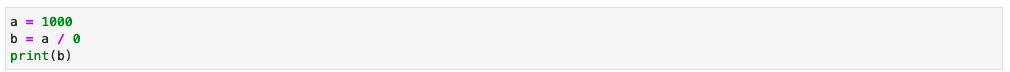
\includegraphics[width=1.0\linewidth]{img/division-by-zero.png}};
          \end{tikzpicture}
          \\
          \vspace{0.1cm}
          \begin{tikzpicture}
            \node[anchor=south west,inner sep=0] at (0,0) {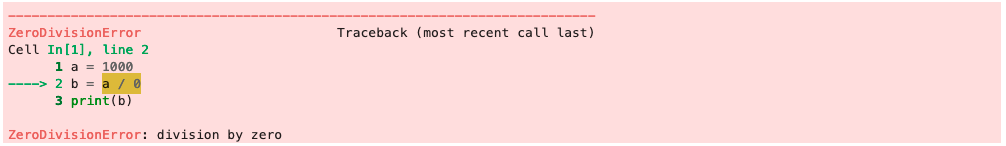
\includegraphics[width=1.0\linewidth]{img/exception.png}};
          \end{tikzpicture}
        \end{itemize}
      \end{frame}
      
       \begin{frame}{\trans{Behandlung von Exceptions}{Exception Handling}}
        \begin{itemize}
          \item \trans
          {Wir können \textbf{Try}- und \textbf{Except}-Klauseln verwenden, um Exceptions zu behandeln.}
          {We can use \textbf{try} and \textbf{except} clauses to handle exceptions.}
           \item \trans
           {Eine try-Anweisung kann mehr als eine except-Klausel haben, um Handler für verschiedene Exceptions anzugeben.}
           {A try statement can have more than once except clause, to specify handlers for different exceptions.}
           \item \trans
           {Es wird jedoch höchstens ein Handler ausgeführt.}
           {However, at most one handler will be executed.}
            \\
          \vspace{0.3cm}
          \begin{tikzpicture}
            \node[anchor=south west,inner sep=0] at (0,0) {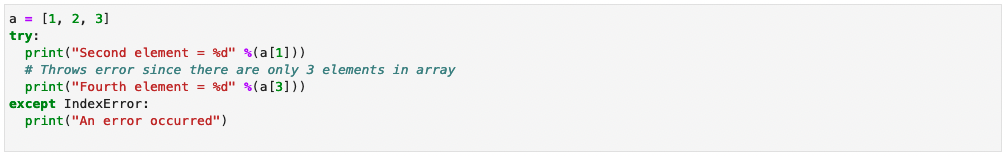
\includegraphics[width=1.0\linewidth]{img/try-except.png}};
          \end{tikzpicture}
          {\footnotesize \textbf{Output:}}
           \\
            \vspace{0.1cm}
          \begin{tikzpicture}
            \node[anchor=south west,inner sep=0] at (0,0) {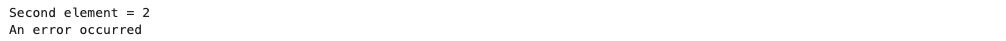
\includegraphics[width=1.0\linewidth]{img/try-except-output.png}};
          \end{tikzpicture}
        \end{itemize}
      \end{frame}
      
      \begin{frame}{\trans{Finally}{Finally}}
        \begin{itemize}
          \item \trans
          {\textbf{finally} definiert Code, der immer nach einem Try-and-Except-Block ausgeführt wird, unabhängig davon, ob eine Exception ausgelöst wird oder nicht.}
          {\textbf{finally} defines code that is always executed after a try and except block, independently if an exception is raised or not.}
           \\
          \vspace{0.3cm}
          \begin{tikzpicture}
            \node[anchor=south west,inner sep=0] at (0,0) {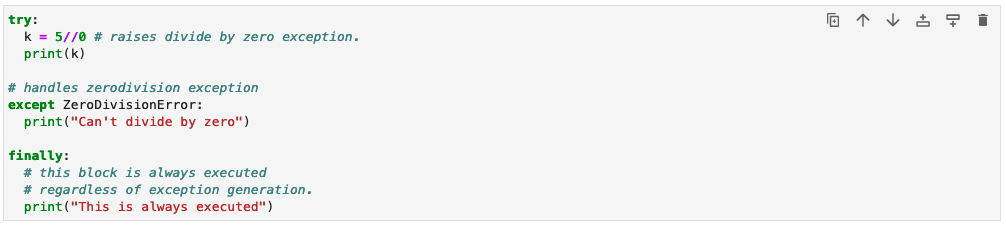
\includegraphics[width=1.0\linewidth]{img/finally.png}};
          \end{tikzpicture}
          {\footnotesize \textbf{Output:}}
           \\
            \vspace{0.1cm}
          \begin{tikzpicture}
            \node[anchor=south west,inner sep=0] at (0,0) {
\includegraphics[width=1.0\linewidth]{img/finally-output.png}};
          \end{tikzpicture}
        \end{itemize}
      \end{frame}
      
      \begin{frame}{\trans{Benutzerdefinierte Exceptions}{User-Defined Exceptions}}
        \begin{itemize}
          \item \trans
          {Man kann seine eigenen Exceptions erstellen, indem man eine neue Klasse erstellt.}
          {You can create your own exceptions by creating a new class.}
          \item \trans
          {Neue Exceptions müssen von der Klasse \textbf{Exception} abgeleitet werden.}
          {New exceptions must derive from the \textbf{Exception} class.}
           \\
          \vspace{0.3cm}
          \begin{tikzpicture}
            \node[anchor=south west,inner sep=0] at (0,0) {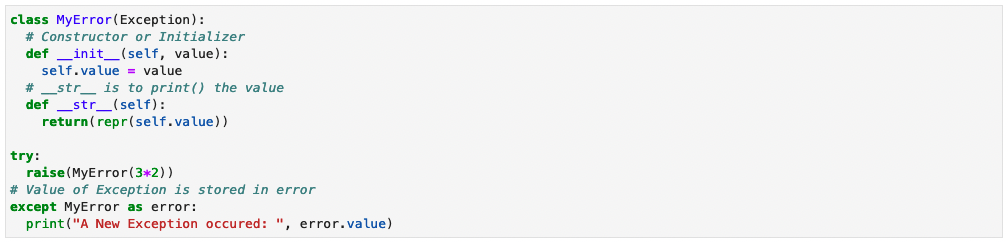
\includegraphics[width=1.0\linewidth]{img/custom.png}};
          \end{tikzpicture}
          {\footnotesize \textbf{Output:}}
           \\
            \vspace{0.1cm}
          \begin{tikzpicture}
            \node[anchor=south west,inner sep=0] at (0,0) {
\includegraphics[width=1.0\linewidth]{img/custom-output.png}};
          \end{tikzpicture}
        \end{itemize}
      \end{frame}



\section{\trans{In-class Exercises}{In-class Exercises}}
\sectionframe{}

\begin{frame}[fragile]{\trans{Variablen}{Reading user input}}
\begin{codebox}
\beginlst
word = input("Enter a word : ")
\end{lstlisting}
\end{codebox}
\begin{itemize}
    \item This code writes a text "\texttt{Enter a word : }" on a console and waits for user input.
    \item After the user enters some text, it is stored into variable \texttt{word} as data type string.
\end{itemize}

\end{frame}


\begin{frame}[fragile]{\trans{Variablen}{Reading user input in a loop}}
\begin{codebox}
\beginlst
word = input("Enter a word : ")
  again = True
  while again:
    #Do something with word...
    word = input("Enter a word (or just <ENTER> to stop): ")
    again = len(word) > 0
\end{lstlisting}
\end{codebox}
\begin{itemize}
    \item This code sequentially reads strings from user, and processes them.
    \item If the user enters an empty string, the program terminates.
\end{itemize}

\end{frame}


\begin{frame}[fragile]{\trans{Variablen}{In-class exercise: Palindrome}}

A \textbf{palindrome} is a word that is spelt the same way backwards and forwards.
\vspace{0.5cm}

Write a python program that: 
\begin{itemize}
    \item Sequentially reads words (possibly containing spaces) from user input.
    \item For each word, the program prints whether the word is a palindrome.
    \item If the user enters an empty string, the program terminates.
\end{itemize}
Go to CodeExpert - Code Examples - Exercise 2 - In-class
\vspace{0.5cm}

\textbf{Hint:} a string is a sequence. All sequence operations can be applied to it.

\end{frame}

\begin{frame}[fragile]{\trans{Variablen}{In-class exercise: Count of numbers above average}}
Write a python program with the following input, and output:\footnote{Do this exercise if there is spare time.}

\textbf{Input:} A list \texttt{s} of numbers.\\
\textbf{Output:} The count of numbers in list \texttt{s} that are strictly larger than the average value.

\vspace{0.2cm}
\textbf{Example:}
\texttt{s = [1,1,2,3,4,1]}\\
The average value in list \texttt{s} is equal to 2. There are two numbers in \texttt{s} that are larger than 2: 3, and 4. Therefore, the output should be 2.

\end{frame}



\section{Homework}
\sectionframe{}

\begin{frame}[fragile]{\trans{Variablen}{Exercise 1: Python I}}

On https://expert.ethz.ch/mycourses/SS23/mavt2/exercises
\begin{itemize}
    \item Sum and Maximum
    \item List Comprehension
    \item Dict Comprehension
    \item Crops \& Dictionaries
\end{itemize}
Due date: Monday 06.03.2023, 20:00 CET\\
%\vspace{0.5cm}
\textbf{NO HARDCODING}

\end{frame}


{
\setbeamercolor*{frametitle}{bg=textbg}
\begin{frame}
	\begin{center}
	\Huge{\trans{Fragen?}{Questions?}}
	\end{center}
\end{frame}
}

\end{document}
